\documentclass[11pt,handout,aspectratio=169]{beamer}


%%%%%%%%% GENERAL PACKAGES
%\usepackage{xcolor}
%\usepackage{pdfpages}
%\usetheme[progressbar=frametitle]{metropolis}
%\setbeamercolor{background canvas}{bg=white}
%\usepackage{appendixnumberbeamer}
%\usepackage{booktabs}
%\usepackage[scale=2]{ccicons}
%\usepackage{pgfplots}
%\usepgfplotslibrary{dateplot}
%\usepackage{xspace}
%\newcommand{\themename}{\textbf{\textsc{metropolis}}\xspace}
%\usepackage[absolute,overlay]{textpos}

%%%%%%%%% COLOR THEME

% Define some colors:
\definecolor{DarkFern}{HTML}{407428}
\definecolor{DarkCharcoal}{HTML}{4D4944}
\definecolor{AlertColor}{RGB}{89,124,158}
\definecolor{HighLight}{RGB}{96,95,134}
\definecolor{Important}{RGB}{234,122,133}
\definecolor{Yellow}{HTML}{00539C}
\colorlet{Fern}{DarkFern!85!white}
\colorlet{Charcoal}{DarkCharcoal!85!white}
\colorlet{LightCharcoal}{Charcoal!50!white}
\colorlet{HighLight2}{AlertColor}
\colorlet{DarkRed}{red!70!black}
\colorlet{DarkBlue}{blue!70!black}
\colorlet{DarkGreen}{green!70!black}
\definecolor{RoyalBlue}{HTML}{00539C}
\definecolor{Peach}{HTML}{EEA47F}
\definecolor{ForestGreen}{HTML}{2C5F2D}
\definecolor{MossGreen}{HTML}{E8FCC9}
% Use the colors:
\setbeamercolor{title}{fg=Fern}
\setbeamercolor{frametitle}{fg=MossGreen,bg=ForestGreen}
\setbeamercolor{normal text}{fg=Charcoal!70!black}
\setbeamercolor{block title}{fg=black,bg=Fern!25!white}
\setbeamercolor{block body}{fg=black,bg=Fern!10!white}
\setbeamercolor{block title alerted}{fg=black,bg=DarkRed!25!white}
\setbeamercolor{block body alerted}{fg=black,bg=DarkRed!10!white}
\setbeamercolor{alerted text}{fg=DarkRed}
\setbeamercolor{itemize item}{fg=Charcoal}



%%%%%%%%% OTHER COMMANDS
\newcommand{\indep}{\perp\!\!\! \perp}
\newcommand{\comment}[1]{}
\newcommand{\bs}{\boldsymbol}
\newcommand{\tr}{\text{trace}}
\newcommand{\sgn}{{\rm sgn}}
\def\T{\top}
%\newcommand{\det}{\text{det}}
\newcommand{\var}{\mathrm{var}}
\newcommand{\cC}{{\cal C}}
\newcommand{\cG}{{\cal G}}
\newcommand{\cV}{{\cal V}}
\newcommand{\cE}{{\cal E}}
\newcommand{\cM}{{\cal M}}
\newcommand{\cP}{{\cal P}}
\newcommand{\cX}{{\cal X}}
\newcommand{\cY}{{\cal Y}}
\newcommand{\X}{\mathbf{X}}
\newcommand{\Y}{\mathbf{Y}}
\newcommand{\x}{\mathbf{x}}
\newcommand{\y}{\mathbf{y}}
\newcommand{\z}{\mathbf{z}}

\newcommand{\argmin}{\operatornamewithlimits{argmin}}
\newcommand{\eps}{\varepsilon}
\newcommand{\<}{\langle}
\renewcommand{\>}{\rangle}


\setbeamertemplate{itemize subitem}{\tiny\raise1.5pt\hbox{\donotcoloroutermaths$\blacktriangleright$}}
\setbeamertemplate{itemize subsubitem}{\tiny\raise1.5pt\hbox{\donotcoloroutermaths$\blacktriangleright$}}
\setbeamertemplate{enumerate item}{\insertenumlabel.}
\setbeamertemplate{enumerate subitem}{\insertenumlabel.\insertsubenumlabel}
\setbeamertemplate{enumerate subsubitem}{\insertenumlabel.\insertsubenumlabel.\insertsubsubenumlabel}
\setbeamertemplate{enumerate mini template}{\insertenumlabel}

\newcommand{\TODO}[1]{{\color{red}{[TODO: #1]}}}


\newcommand{\R}{\mathbb R}
\newcommand{\E}{\mathbb E}
\renewcommand{\P}{\mathbb P}


\DeclareMathOperator*{\cov}{cov}


\newsavebox{\zerobox}
\newenvironment{nospace}
{\par\edef\theprevdepth{\the\prevdepth}\nointerlineskip
  \setbox\zerobox=\vtop to 0pt\bgroup
  \hrule height0pt\kern\dimexpr\baselineskip-\topskip\relax
}
{\par\vss\egroup\ht\zerobox=0pt \wd\zerobox=0pt \dp\zerobox=0pt
  \box\zerobox}

\usepackage{soul}
\makeatletter
\let\HL\hl
\renewcommand\hl{%
  \let\set@color\beamerorig@set@color
  \let\reset@color\beamerorig@reset@color
  \HL}
  \makeatother


\title[STA437-Week1]{STA 437/2005: \\ Methods for Multivariate Data}
\subtitle[]{Weeks 9-10: Non-linear Dimension Reduction Techniques}
\author[Piotr Zwiernik]{Piotr Zwiernik}
\institute[UofT]{University of Toronto}
\date{}


%\usepackage{Sweave}

\begin{document}

\maketitle


\begin{frame}{Why Principal Component Analysis may not be enough?}
  PCA struggles with non-linear relationships. \\[2mm]
  High-dimensional datasets often lie on low-dimensional manifolds. \\[2mm]
  Linear projections may destroy these geometric information.
  \begin{center}
 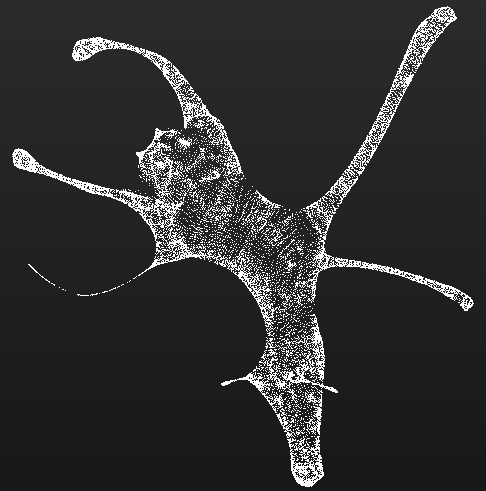
\includegraphics[height=4cm]{pics/exUMAP1}  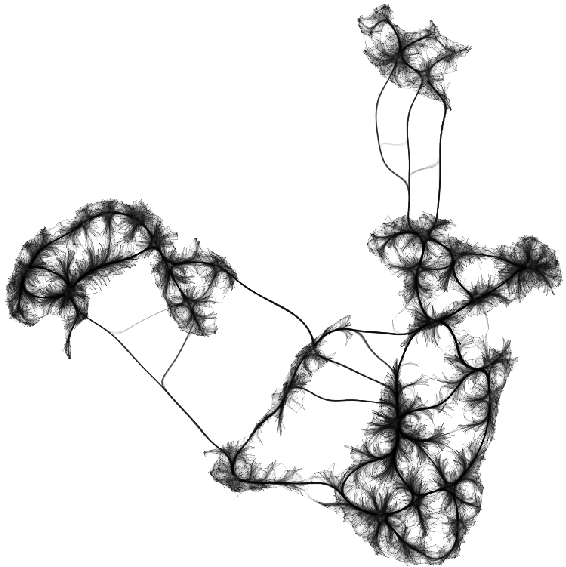
\includegraphics[height=4cm]{pics/exUMAP2}
\includegraphics[height=4cm]{pics/exUMAP3}	
  \end{center}
  We will now discuss four popular non-linear dimensionality reduction techniques: multi-dimensional scaling, spectral embedding, UMAP, and Autoencoders.
 \end{frame}

\begin{frame}{}
	\begin{center}
		\alert{\Huge Multi-dimensional Scaling (MDS)}
	\end{center}
	\begin{itemize}
		\item In its classical version this is essentially PCA.
		\item MDS allows us to introduce some fundamental concepts.
	\end{itemize}
\end{frame}

% Slide: Problem Setup
\begin{frame}{Problem Setup}
Consider $n$ objects and  a measure $\delta_{ij}\geq 0$ of their dissimilarity (small if similar); $\delta_{ii}=0$.\\[3mm]
Define $\Delta=(\delta_{ij})\in \R^{n\times n}$: $\delta_{ii}=0$ for all $i$, $\delta_{ij}\geq 0$ for all $i\neq j$. \\[5mm]

In \textcolor{blue}{classical MDS}: there exist $\x_1,\ldots,\x_n\in \R^m$ such that $\delta_{ij}=\|\x_i-\x_j\|$.\\[5mm]
 \hl{In general, there need not be a Euclidean distance defining this metric.}
\begin{alertblock}{Multidimensional Scaling}
	Find a configuration of points $\y_1,\ldots,\y_n$ in $\R^d$ ($d<\!\!<n$) such that:
	$$
	\|\y_i-\y_j\|\;\approx\;\delta_{ij}.
	$$ 
\end{alertblock}
The solution for classical MDS is particularly simple.
\end{frame}

% Slide: Distance Matrix Algebra
\begin{frame}{Classical MDS: $\delta_{ij}=\|\x_i-\x_j\|$}
If $\delta_{ij}=\|\x_i-\x_j\|$, we have:
\[\delta_{ij}^2 \;=\; (\mathbf{x}_i - \mathbf{x}_j)^{\top}(\mathbf{x}_i - \mathbf{x}_j)\;=\;(\X\X^\top)_{i,i}+(\X\X^\top)_{j,j}-2(\X\X^\top)_{i,j}.\]
The Hadamard product $\Delta\odot\Delta=[\delta_{ij}^2]$ can be written as:
	\[\Delta \odot \Delta = \mathrm{diag}(\mathbf{X}\mathbf{X}^{\top}) \mathbf{1} \mathbf{1}^{\top} + \mathbf{1} \mathbf{1}^{\top} \mathrm{diag}(\mathbf{X}\mathbf{X}^{\top}) - 2\mathbf{X}\mathbf{X}^{\top}\]
	Reintroducing the centering matrix $H = I_n - \frac{1}{n}\mathbf{1}\mathbf{1}^{\top}$, we obtain
	\[B \;:=\; -\frac{1}{2} H (\Delta \odot \Delta) H\;=\;H\X (H\X)^\top \;=\;\tilde\X\tilde\X^\top.\]
	This matrix contains all inner products $\tilde\x_i^\top\tilde\x_j$ for $1\leq i,j\leq n$.
\end{frame}

% Slide: Centering the Matrix
\begin{frame}{Classical MDS (2)}
Let $\Y\in \R^{n\times d}$ be the matrix with projected data $\y_1,\ldots,\y_n\in \R^d$. \\[3mm]
We want to make sure $B=\tilde\X\tilde\X^\top\approx \Y\Y^\top=:\textcolor{blue}{M}$
\begin{itemize}
	\item In this way $\|\y_i-\y_j\|\approx \|\x_i-\x_j\|$ as desired. 
	\item One way to assure this is to minimize $\sum_{i,j}(\tilde\x_i^\top \tilde\x_j-\y_i^\top\y_j)^2=\|B-\textcolor{blue}{M}\|^2_F$.
	\item The Frobenius norm $\|A\|_F=\sqrt{\sum_{i,j} A_{ij}^2}$.\\[3mm]
\end{itemize}
Note that ${\rm rank}(\textcolor{blue}{M})\leq d$ but otherwise $\textcolor{blue}{M}\in \R^{n\times n}$ is arbitrary.\\[3mm]
\textbf{Optimization problem:} Minimize $\|B-\textcolor{blue}{M}\|^2_F$ subject to ${\rm rank}(\textcolor{blue}{M})\leq d$.
\end{frame}

\begin{frame}{Classical MDS (3)}
\textbf{Optimization problem:} Minimize $\|B-\textcolor{blue}{M}\|^2_F$ subject to ${\rm rank}(\textcolor{blue}{M})\leq d$.\\[5mm]
	Let $B=V \Lambda V^\top$ be the spectral decomposition with ${\rm diag}(\Lambda)$ non-increasing.
\begin{alertblock}{Eckart-Young Theorem}
The optimal $\textcolor{blue}{M}$ satisfies $\widehat M=V_d\Lambda_d V_d^\top$, where 
\begin{itemize}
	\item $\Lambda_d={\rm diag}(\lambda_1,\ldots,\lambda_d)$ has $d$ largest eigenvalues of $B$.
	\item $V_d\in \R^{n\times d}	$ contains the first $d$ columns of $V$. 
\end{itemize}
We then take $\Y=V_d\Lambda_d^{1/2}$, which gives us our low-dimensional embedding.
\end{alertblock}
\bigskip 

We next show that this is the same answer we would get using PCA!
\end{frame}

\begin{frame}{Duality Between MDS and PCA}
Both methods rely on the singular value decomposition (SVD) of $\tilde \X=H\mathbf{X}=VDU^\top$.\\[5mm]
Here is the key insight:
\begin{itemize}
    \item \textbf{PCA}: Finds principal components from the eigenvectors of $\tilde\X^{\top}\tilde\X=U (D^\top D) U^\top$.
    \item \textbf{MDS}: Finds embeddings from the eigenvectors of $\tilde\X\tilde\X^{\top}=V(DD^\top) V^\top$.\\[5mm]
\end{itemize}
The columns of $U$ are the principal directions and the scores $\y_1,\ldots,\y_n$ are taken as the first $d$ columns of $\tilde\X U=VD$.\\[5mm]


As a result, $\y_1,\ldots,\y_n$ are precisely the points obtained by classical MDS. 
\end{frame}

\begin{frame}{}
    \begin{center}
        \alert{\Huge Spectral Embedding (aka Laplacian Eigenmaps)}
    \end{center}
\end{frame}

% Slide: Problem Setup
\begin{frame}{Main ideas}
Data: $\x_1,\ldots,\x_n\in \R^m$. Find low dimensional representation $\y_1,\ldots,\y_n\in \R^d$.
\begin{alertblock}{Links to manifold learning}
	We look for a truly nonlinear method that is able to learn the underlying manifold.
\end{alertblock}
The main idea is to keep track of local geometry:\\ 
\qquad $\bullet$\;\hl{The embedding of }\hl{$\x_i$}\hl{ should depend mostly on points close to }\hl{$\x_i$}.
\begin{block}{How to keep track of the local geometry in the data?}
Construct a weighted graph $G=(V,E,W)$:
    \begin{itemize}
        \item Vertices $V=\{1,2,\ldots,n\}$ (data points).
        \item Edges $E$ based on proximity (e.g., $k$-nearest neighbors or $\epsilon$-neighborhood).
        \item Weights $W_{ij}$ measure similarity, e.g. $W_{ij}=1$ or $W_{ij}=\exp(-\|\x_i-\x_j\|^2/2\sigma^2)$.
    \end{itemize}
\end{block}
If $ij\notin E$ we always set $W_{ij}=0$, also $W_{ii}=0$ for all $i=1,\ldots,n$.
\end{frame}

% Slide: Graph Laplacian
\begin{frame}{Graph Laplacian}
\alert{Graph Laplacian} is the main object encoding the ``geometry of the data''. 
\begin{alertblock}{The Laplacian matrix $L\in \mathbb S^n$ encodes the structure of the graph:}
	\begin{itemize}
    \item Degree matrix $D$ (diagonal): $D_{ii}=\sum_j W_{ij}$, $i=1,\ldots,n$.
    \item Graph Laplacian: $L = D - W$, where $W$ is the weight matrix $W=(W_{ij})$.
    \item Normalized Laplacian: $L_{\textsc{n}} = D^{-1/2} L D^{-1/2}$.
\end{itemize}
\end{alertblock}
\alert{\textbf{Important exercise:}} Show \hl{$\x^\top L\x=\tfrac12\sum_{i,j} W_{ij}(x_i-x_j)^2$} for all $\x\in \R^n$.\\[4mm]
Properties of $L$:
\begin{itemize}
    \item $L$ is positive semi-definite.
    \item $L\mathbf 1=\mathbf 0$, that is, smallest eigenvalue is zero with eigenvector $\mathbf{1}$.
    \item If $G$ is connected ${\rm rank}(L)=n-1$.
\end{itemize}
\end{frame}

% Slide: Optimization Problem
\begin{frame}{The key idea behind spectral embedding}
Fix $d$. The embedding $\y_1,\ldots,\y_n\in \R^d$ is obtained by minimizing:
\[\frac{1}{2}\sum_{i=1}^n\sum_{j=1}^n W_{ij}\|\y_i - \y_j\|^2\]
\begin{alertblock}{Key insight}
	High $W_{ij}$ enforces small $\|\y_i-\y_j\|$.
\end{alertblock}
Note: This is still not well defined because $\y_1=\ldots=\y_n=\bs 0$ is a solution so we need to refine this idea a bit.  
\end{frame}


\begin{frame}{Problem reformulation}
Let $\Y\in \R^{n\times d}$ be the embedded data matrix. Recall $L=D-W$ and $L\bs 1=\bs 0$.
\begin{alertblock}{Proposition}
We have:\qquad $\frac{1}{2}\sum_{i,j} W_{ij}\|\y_i - \y_j\|^2 \;=\; \text{tr}(\Y^{\top} L \Y)\;=\;\textcolor{gray}{\text{tr}(\Y^{\top} D \Y)-\text{tr}(\Y^{\top} W \Y)}$
\end{alertblock}
Proof: As for MDS we can show that the matrix $E=[\|\y_i-\y_j\|^2]_{i,j}$ takes the form
$$
E\;=\;{\rm diag}(\Y\Y^\top)\bs 1\bs 1^\top+\bs 1\bs 1^\top{\rm diag}(\Y\Y^\top)-2\Y\Y^\top
$$
and so $\tfrac12 \sum_{i,j}W_{ij}\|\y_i-\y_j\|^2 = \tfrac12\tr(W E)$.\\[2mm]	
$D$ is diagonal and $E$ has zeros on the diagonal and so $\tfrac12\tr(W E)=-\tfrac12\tr(L E)$.\\[2mm]
	Since $L\bs 1=\bs 0$ we get also that $-\tfrac12\tr(L E)=\tr(L\Y\Y^\top)$. 
\end{frame}

\begin{frame}{Introducing constraints to the optimization problem}
	\begin{block}{Constraint 1 (Fixing scale)}
		To avoid trivial solutions it is convenient to assume $\Y^\top D \Y=I_d$.\\[2mm]
%		\qquad$\bullet$ \quad we  also assume $\Y^{\top} D \mathbf{1} = \mathbf{0}$.
	\end{block}
Defining $\tilde\Y=D^{1/2}\Y$ we get $\tilde\Y^\top \tilde\Y=I_d$ (orthonormal \alert{columns} $\tilde\y_1,\ldots,\tilde\y_d$).\\[3mm]
Now $\tr(\Y^\top L\Y)=\tr(\tilde\Y^\top L_{\textsc{n}}\tilde\Y)=\sum_{i=1}^d \tilde\y_i^\top L_{\textsc{n}}\tilde\y_i$.\\[3mm]
From PCA: the optimum given by eigenvectors of $L_{\textsc{n}}$ for \alert{smallest} eigenvalues.\\[2mm] 
Note that $L_{\textsc{n}} D^{1/2}\bs 1=D^{-1/2}L\bs 1=\bs 0$ so $\tilde\y_0:=D^{1/2}\bs 1$ is a zero-eigenvector.
\begin{block}{Constraint 2: $\tilde\y_0\perp \tilde \y_i$ for $i=1,\ldots,n$}
		In addition we assume $\tilde\Y^\top D^{1/2}\bs 1=\Y^{\top} D \mathbf{1} = \mathbf{0}$.
\end{block}
\begin{alertblock}{}
\alert{Spectral embedding}:	minimize $\tr(\Y^\top L \Y)$ subject to $\Y^\top D\Y=I_d$ and $\Y^{\top} D \mathbf{1} = \mathbf{0}$
\end{alertblock}

\end{frame}

% Slide: Example (Twisted Curve)

\begin{frame}{Example: Twisted curve}
Consider datapoints lying on the twisted curve as on the picture below:
	\begin{center}
		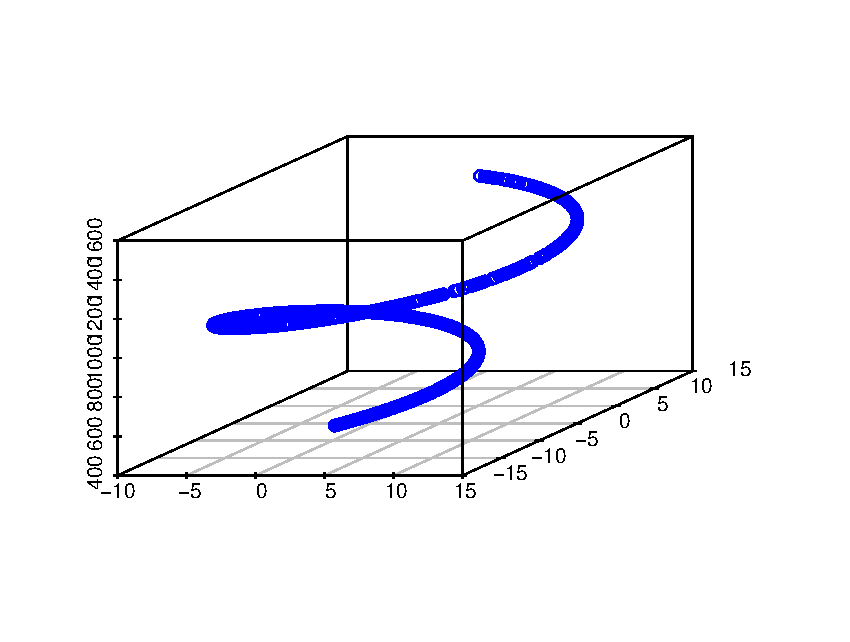
\includegraphics[scale=.7]{pics/twisted.pdf}
	\end{center}
We now represent these data in 2D comparing PCA and Laplacian Eigenmaps.
\end{frame}

\begin{frame}{}
\begin{itemize}
    \item \textbf{PCA}: Projects data linearly, collapsing structure.
    \item \textbf{Laplacian Eigenmaps}: Preserves local geometry, unfolding the manifold.
\end{itemize}
\begin{center}
    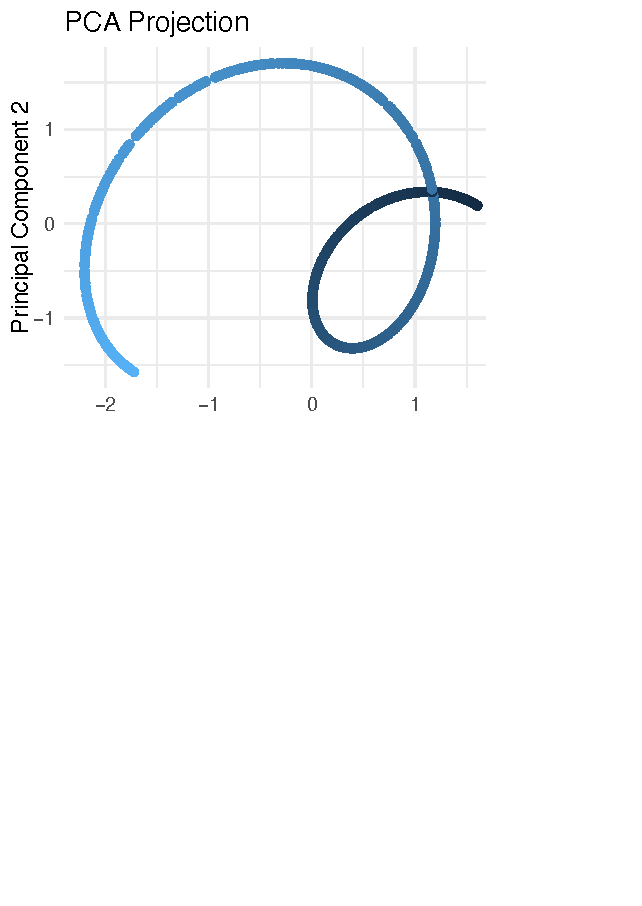
\includegraphics[width=0.45\textwidth]{pics/twistedA.pdf}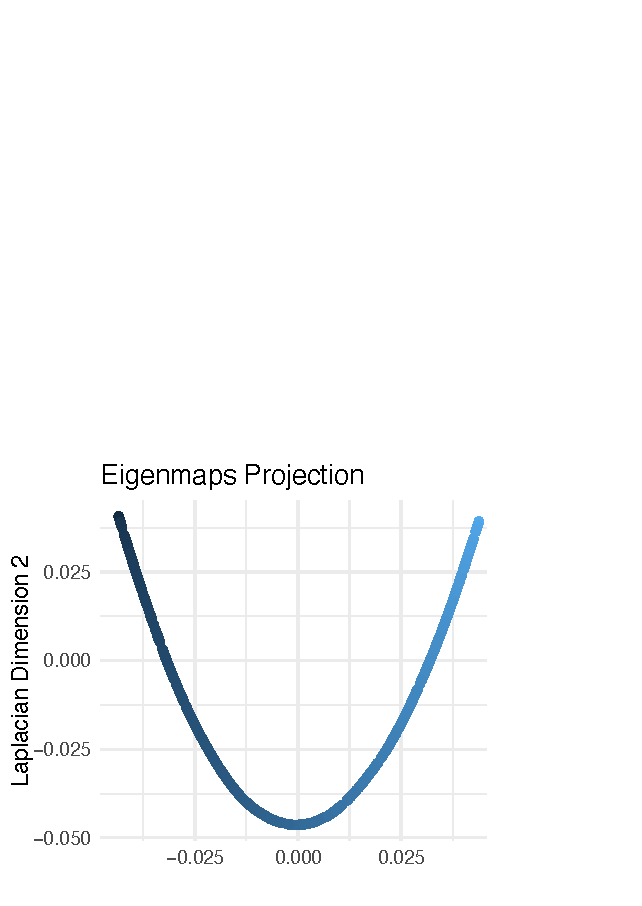
\includegraphics[width=0.45\textwidth]{pics/twistedB.pdf}
\end{center}
Note that PCA joins points that are far from each other in the original dataset.
\end{frame}

\begin{frame}{}
    \begin{center}
        \alert{\Huge Uniform Manifold Approximation and Projection (UMAP)}
    \end{center}
    \begin{itemize}
    \item This is a popular, state-of-the-art method. 
    	\item It relies on various choices that are not fully theoretically justified. 
    	\item We provide a high level overview.
    \end{itemize}
\end{frame}

% Slide: Introduction to UMAP
\begin{frame}{Introduction to UMAP}
UMAP is a nonlinear dimensionality reduction technique that improves on eigenmaps.\\[4mm]
\textbf{Advantages over PCA, MDS, and Eigenmaps:}
    \begin{itemize}
    \item Has manifold learning abilities.\\[3mm]
        \item Balances local and global structure.\\[3mm]
        \item Scales efficiently to large datasets.\\[3mm]
        \item More robust to parameter choices.\\[5mm]
    \end{itemize}
UMAP is a state-of-the-art data visualization and pattern discovery tool.
\end{frame}

%% Slide: Key Idea
%\begin{frame}{Key Idea}
%\begin{alertblock}{Goal}
%Embed $\x_1,\ldots,\x_n\in \mathbb{R}^m$ into a lower-dimensional space $\mathbb{R}^d$ ($d<\!\!<m$) such that:
%$$\|\y_i - \y_j\| \approx \|\x_i - \x_j\|.$$
%\end{alertblock}
%\begin{itemize}
%    \item Similar to Laplacian Eigenmaps, UMAP focuses on preserving local neighborhoods.
%    \item UMAP captures both local and global data structure.
%\end{itemize}
%\end{frame}

% Slide: UMAP Algorithm Overview
\begin{frame}{UMAP Algorithm Overview}
The key idea is similar to the spectral embedding.
\begin{enumerate}
    \item \textbf{Construct k-Nearest Neighbor (kNN) Graph}.\\[3mm]
    \item \textbf{Initialize Embedding} using Laplacian Eigenmaps.\\[3mm]
    \item \textbf{Optimize} embedding via stochastic gradient descent (SGD).\\[5mm]
\end{enumerate}
UMAP uses a different loss function than Laplacian Eigenmaps, which makes it, in principle, more robust to parameter choices. 
\end{frame}

% Slide: Step 1 - Data Graph in the Input Space
\begin{frame}{Step 1: Data Graph in the Input Space}
Construct $k$-Nearest Neighbors (kNN) graph; e.g.  with $k=15$.\\[3mm]
Define ``probabilities'' of $i,j$ being connected based on neighbor distances:
    $$p_{j|i} = \exp\left(-\frac{\|\x_i - \x_j\| - \rho_i}{\sigma_i}\right),$$
    where $\rho_i=\min_{k\neq i}\|\x_i-\x_k\|$ and $\sigma_i$ is a scaling factor.\\[3mm]
Symmetrize probabilities:
    $$p_{ij} = p_{j|i} + p_{i|j} - p_{j|i}p_{i|j}.$$
    Note that the closest neighbor gets always connected with pr. 1.
    \begin{itemize}
    	\item This about $p_{ij}$ as edge weights.
    \end{itemize}
\end{frame}

% Slide: Step 2 - Data Graph in the Embedding Space
\begin{frame}{Step 2 and 3: Data Graph in the Embedding Space and matching}
Compute pairwise similarities in low-dimensional space:
\begin{equation}\label{eq:qij}
	q_{ij} = \frac{1}{1 + a\|\y_i - \y_j\|^{2b}},
\end{equation}
    where, by default,  $a \approx 1.929$, $b \approx 0.7915$.\\[4mm]
The matching between the original and the embedded space is probability-inspired.
\begin{alertblock}{Cost Function (Fuzzy Cross-Entropy)}
$$c(\y_1,\ldots,\y_n) = \sum_{i \neq j} \left(p_{ij} \log \frac{p_{ij}}{q_{ij}} + (1 - p_{ij}) \log \frac{1 - p_{ij}}{1 - q_{ij}}\right).$$
Here $c$ depends on $\y_1,\ldots,\y_n$ through $q_{ij}$'s defined in \eqref{eq:qij}.
\end{alertblock}
\begin{itemize}
\item Attractive and repulsive forces to balance local and global structure.
    \item Uses block-coordinate descent to minimize cost.
\end{itemize}
\end{frame}


% Slide: Example - Iris Dataset
\begin{frame}{Example: Iris Dataset}
\begin{itemize}
    \item Comparison of PCA and UMAP on Iris dataset.
    \item PCA struggles to separate classes clearly.
    \item UMAP better preserves local and global structures.
\end{itemize}
\begin{center}
    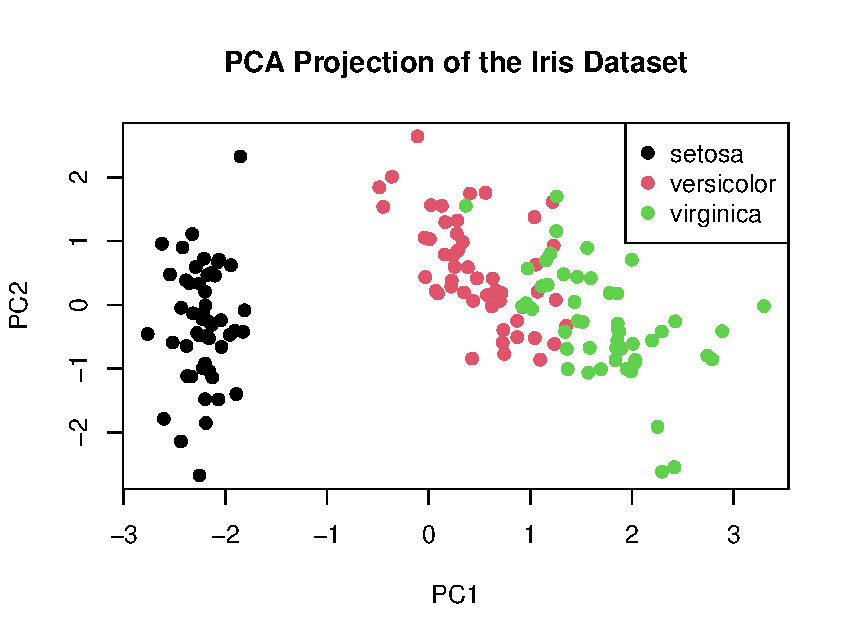
\includegraphics[width=0.4\textwidth]{pics/iris_pca.pdf}
    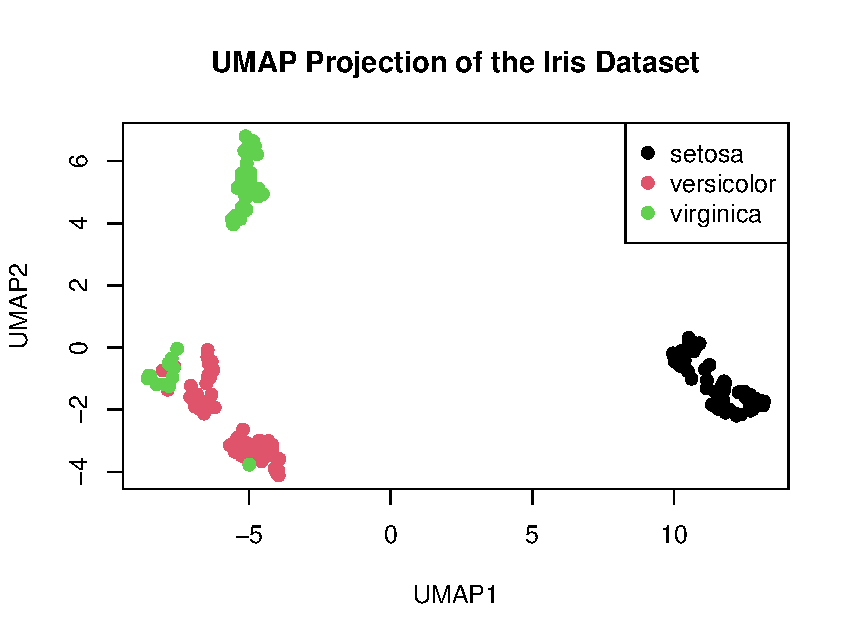
\includegraphics[width=0.4\textwidth]{pics/iris_umap.pdf}
\end{center}
\alert{\textbf{Note:}} Given a new data point UMAP has to be recalculated from scratch!
\end{frame}


\section{Introducing neural networks}

\begin{frame}{}
	\begin{center}
		\alert{\Huge Introducing neural networks}
	\end{center}
	\vspace{1cm}
	We finish by briefly discussing Autoencoders:
	\begin{itemize}
		\item This is a dimension reduction technique based on neural networks.
		\item We ignore computational aspects. 
	\end{itemize}
\end{frame}

\begin{frame}{A Simple Neuron}
For neural nets, we use a simple model for neuron, or \textbf{unit}:

    \begin{center}
      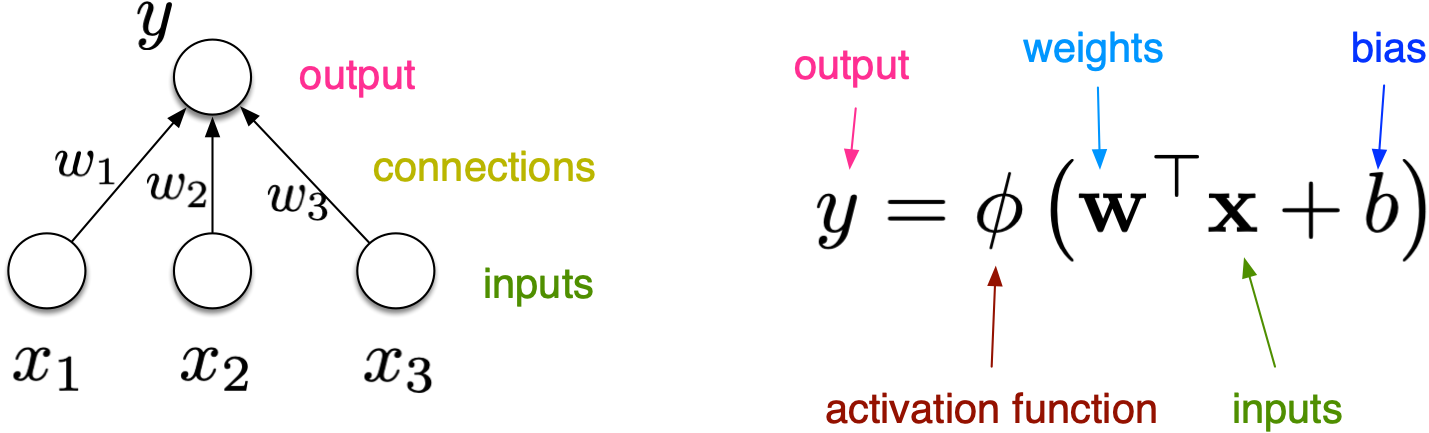
\includegraphics[width=0.8 \textwidth]{pics/neuron2}
    \end{center}
\pause
  \begin{itemize}

  \item By throwing together lots of these simple neuron-like processing units, we can do some powerful computations!
  \end{itemize}
\end{frame}



\begin{frame}{A Feed-Forward Neural Network}
\vspace{5mm}
  \begin{columns}
    \begin{column}{0.45 \linewidth}
      \begin{itemize}
      \item A \alert{directed acyclic graph}
      \item Units are grouped into \alert{layers}
      \end{itemize}
    \end{column}
    \begin{column}{0.65 \linewidth}
      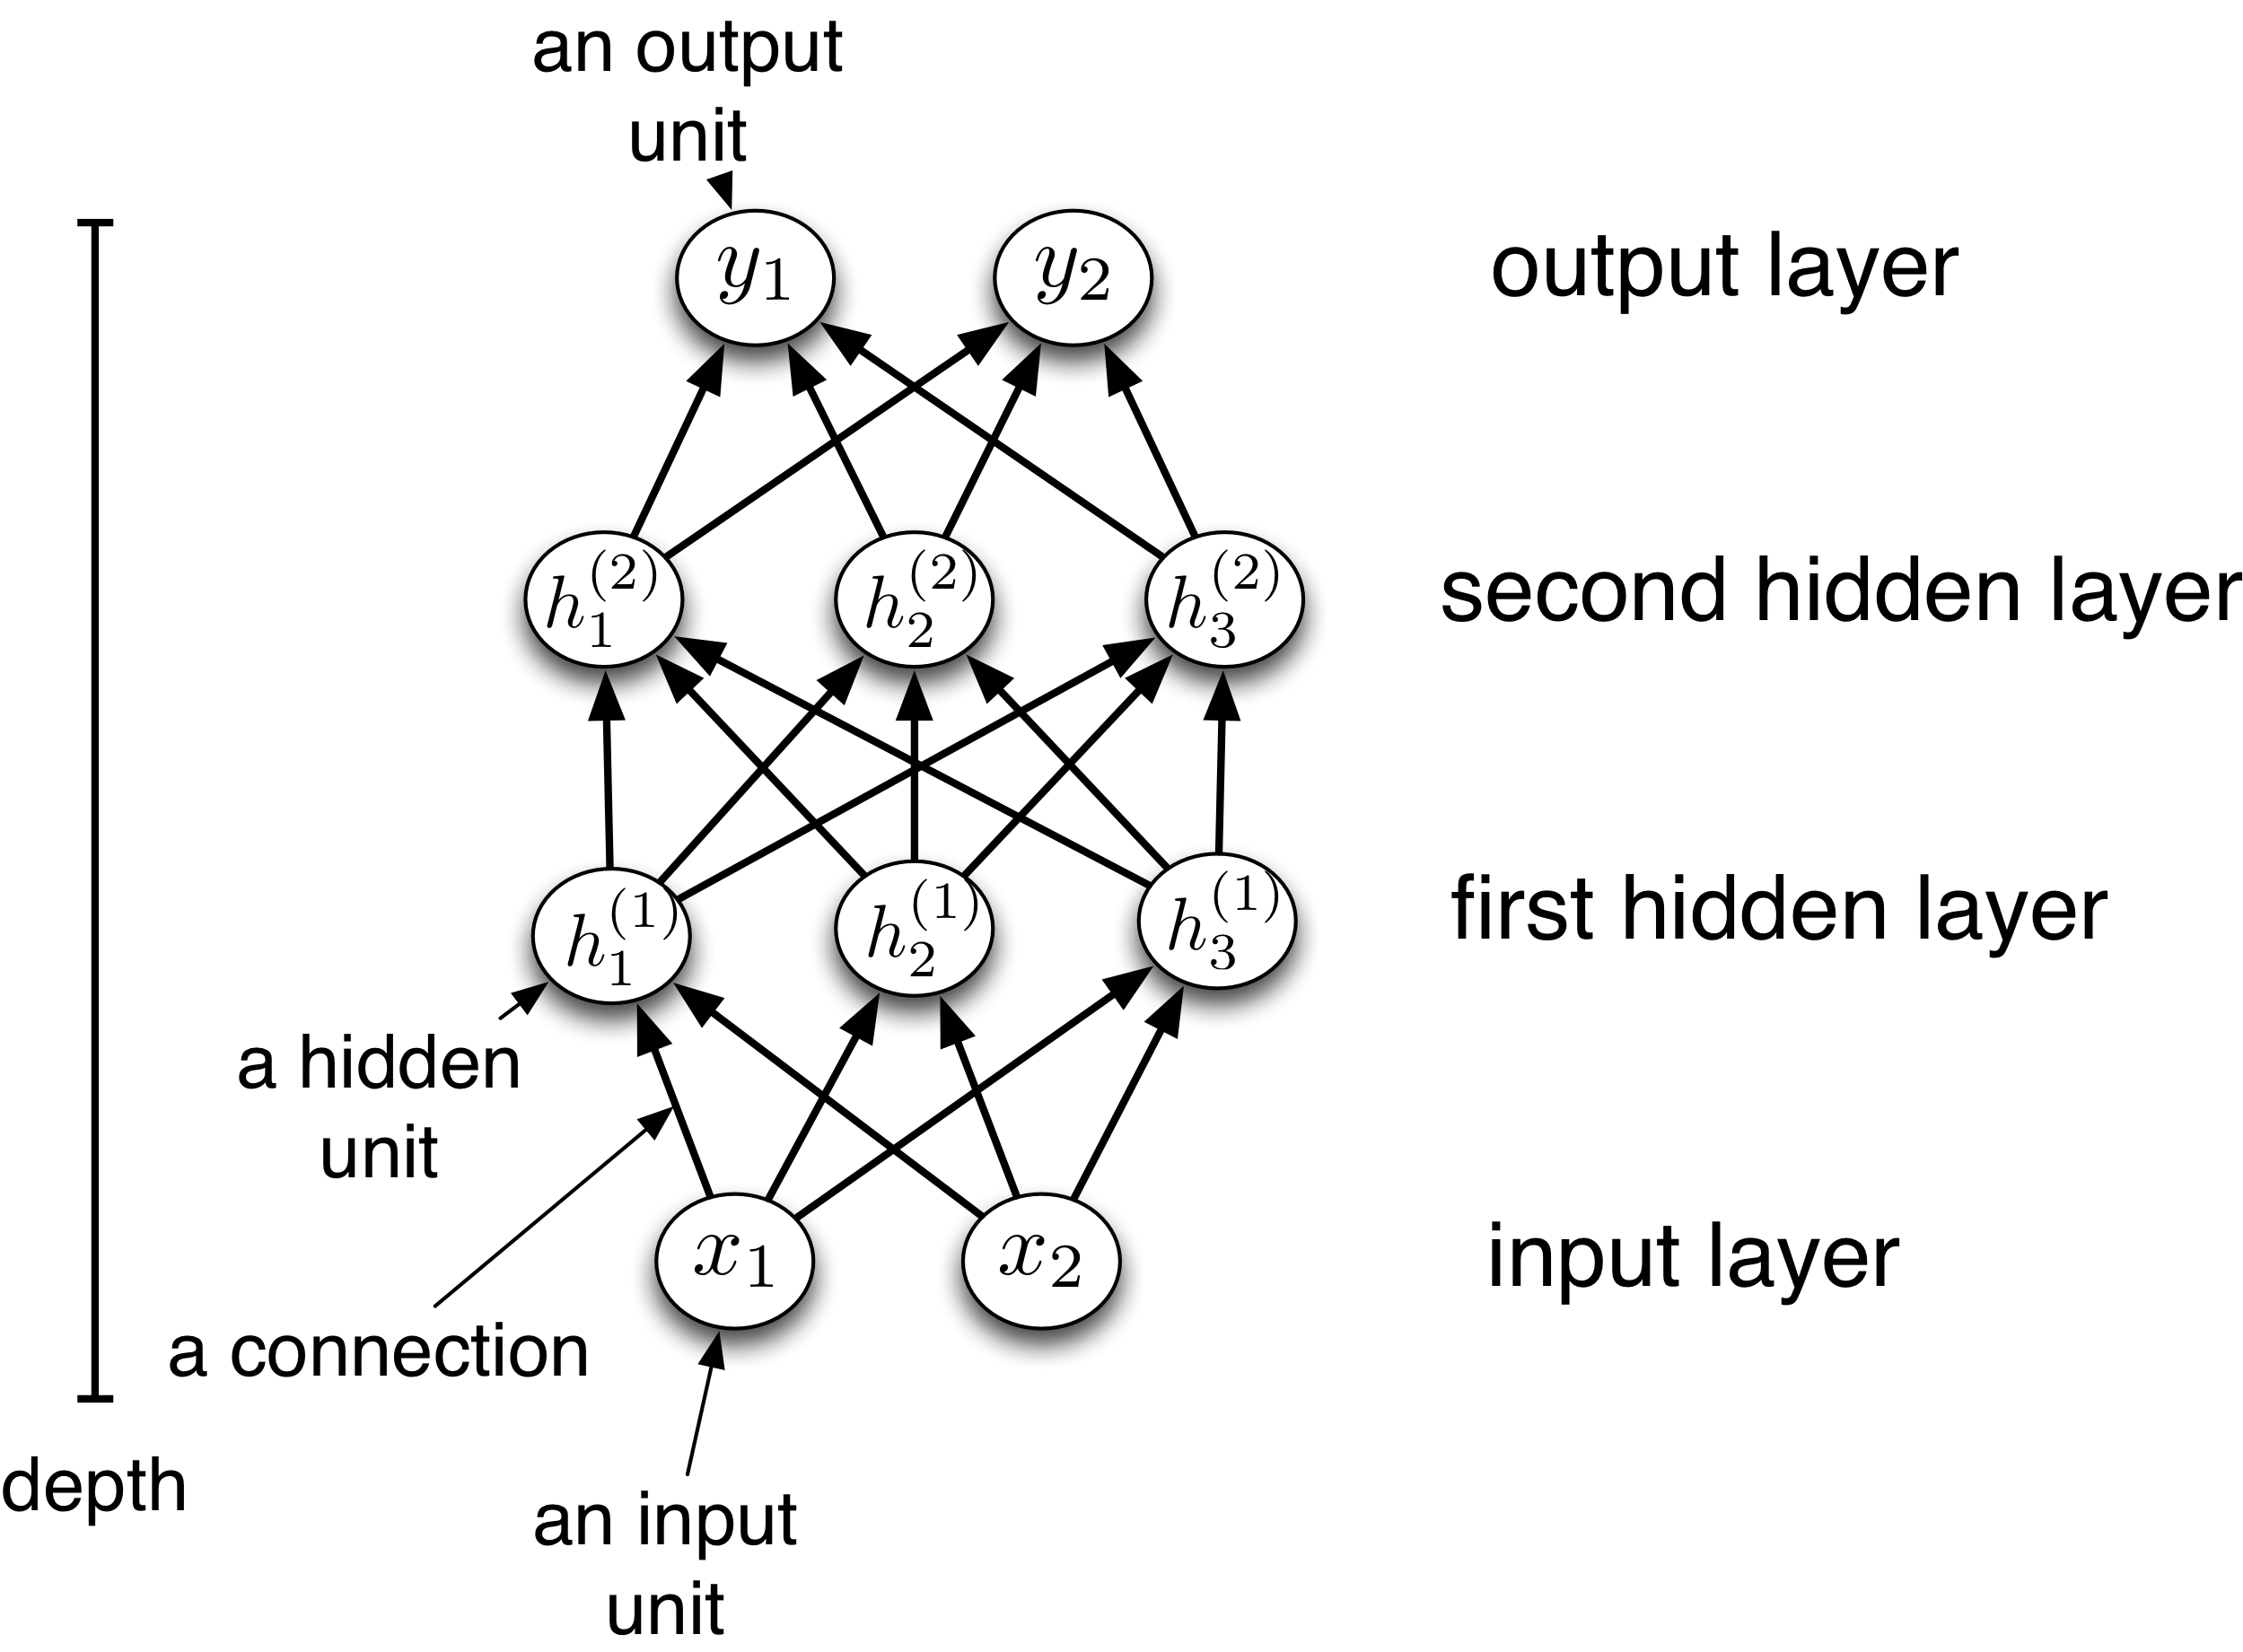
\includegraphics[width=\linewidth]{pics/mlp.png}
    \end{column}
  \end{columns}
\end{frame}

\begin{frame}{Multilayer Perceptrons}
\begin{itemize}
\item A multi-layer network consists of fully connected layers.
\item In a fully connected layer, all input units are connected to 
all output units.
%\item Each hidden layer $i$ connects $N_{i-1}$ input units to $N_{i}$ output
%  units. Weight matrix is $N_i$ x $N_{i-1}$.
\pause
\item The outputs are a function of the input units:
        \[ \y = f(\x) = \phi \left( \mathbf{W} \x + \mathbf{b} \right) \]
        $\phi:\R\to \R$ is applied \alert{component-wise}.
\end{itemize}
\vspace{-4mm}
\begin{center}
  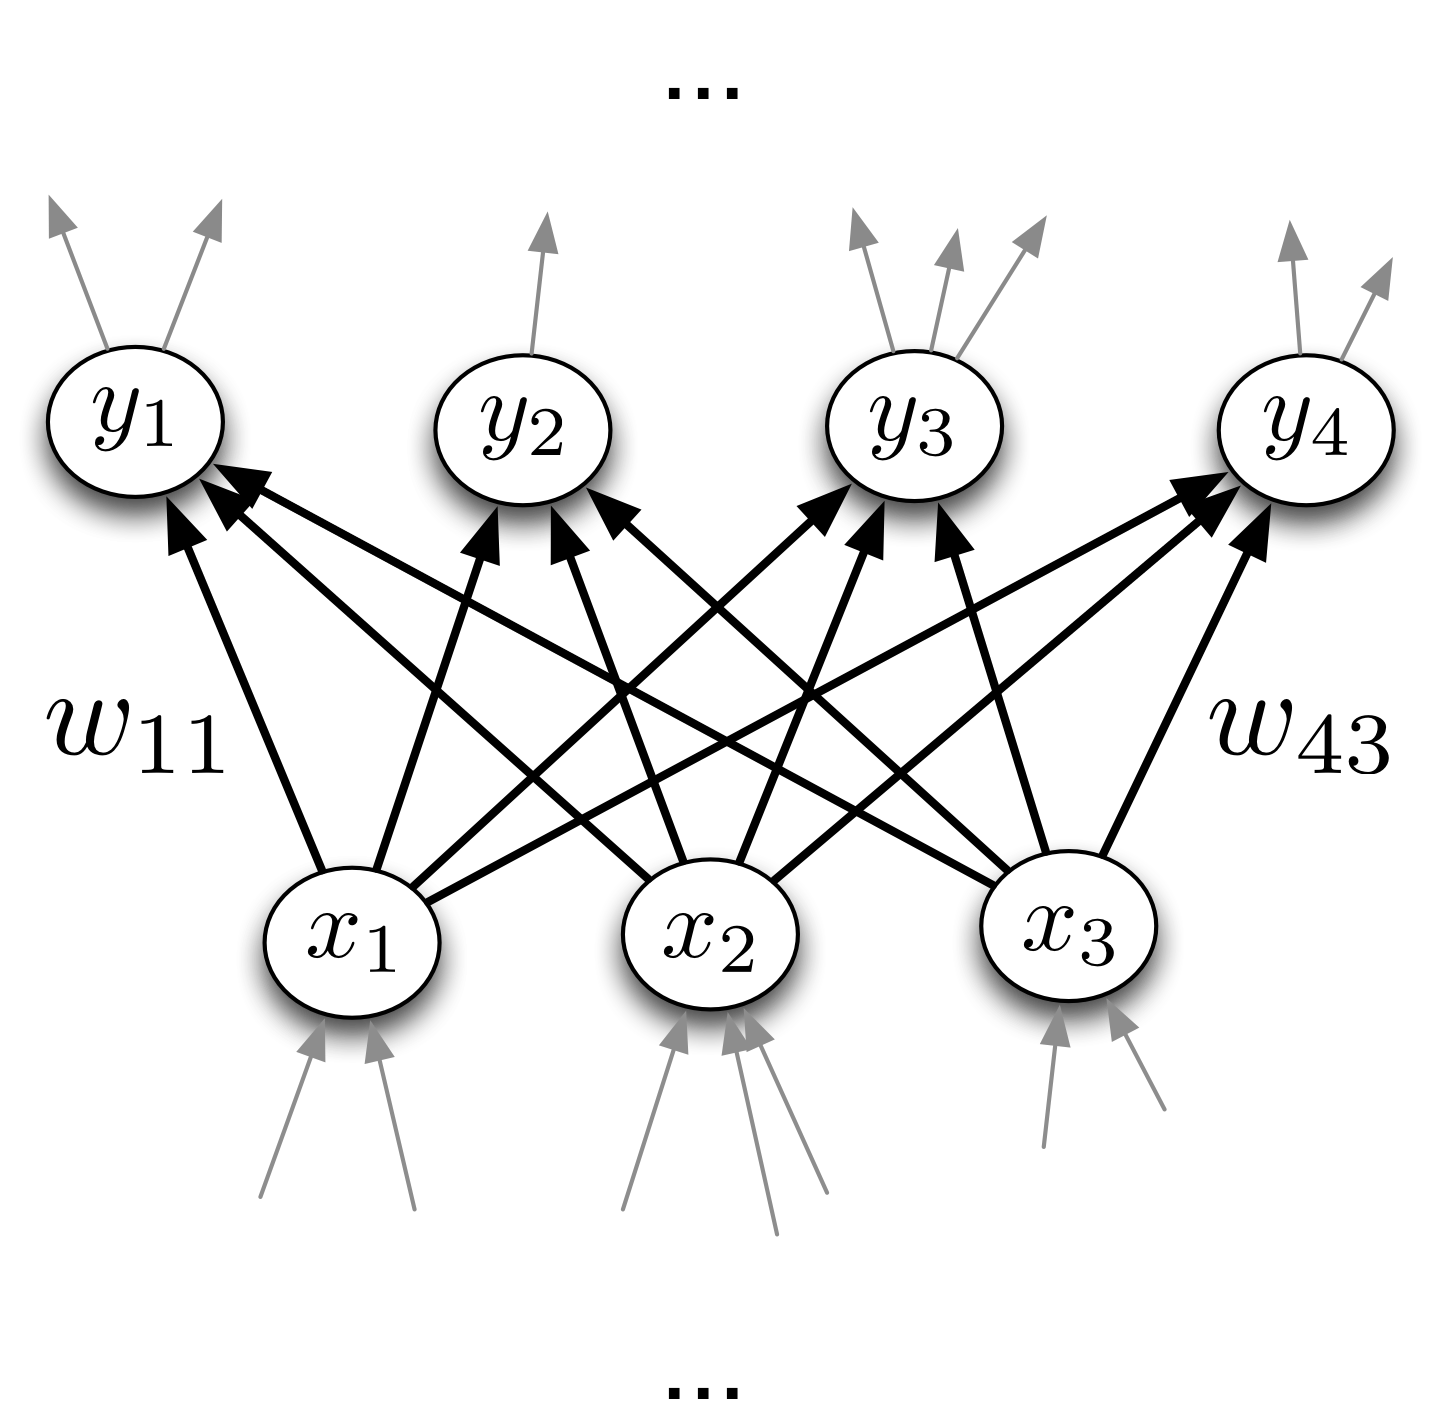
\includegraphics[width=0.3\linewidth]{pics/fc_layer.png}
\end{center}
\end{frame}


\begin{frame}{Some Activation Functions}
  \begin{columns}
    \begin{column}{0.25 \linewidth}
      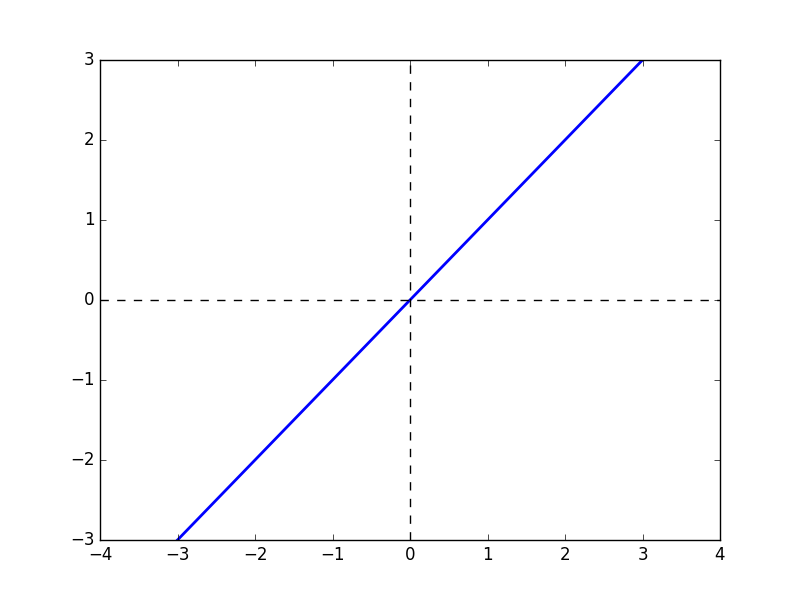
\includegraphics[width=\linewidth]{pics/act_lin.png}
      \begin{center}
        {\bf Identity}
      \end{center}
      \[ \phi(z) = z \]
    \end{column}

    \begin{column}{0.4 \linewidth}
    \centering
      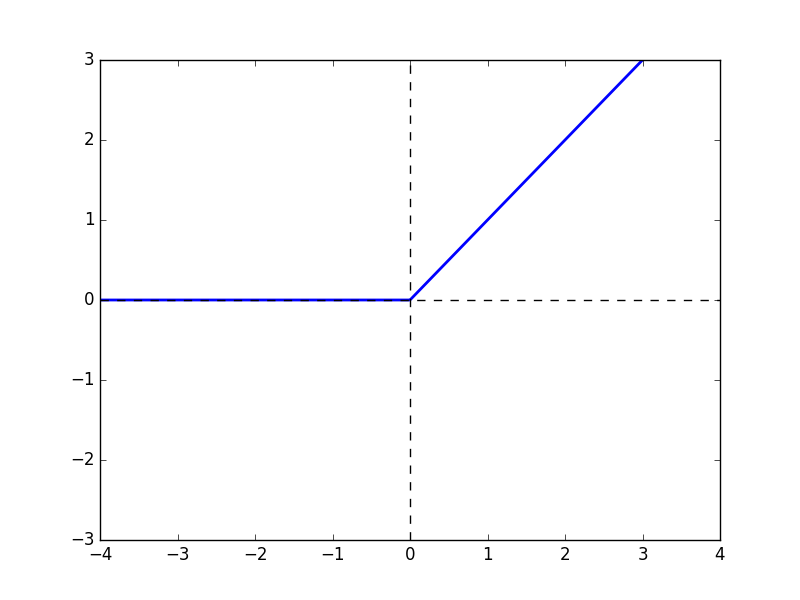
\includegraphics[width=0.8\linewidth]{pics/act_relu.png}
      \begin{center}
        {\bf Rectified Linear Unit} \\
        {\bf (ReLU)}
      \end{center}
      \[ \phi(z) = \max(0, z) \]
    \end{column}

    \begin{column}{0.25 \linewidth}
      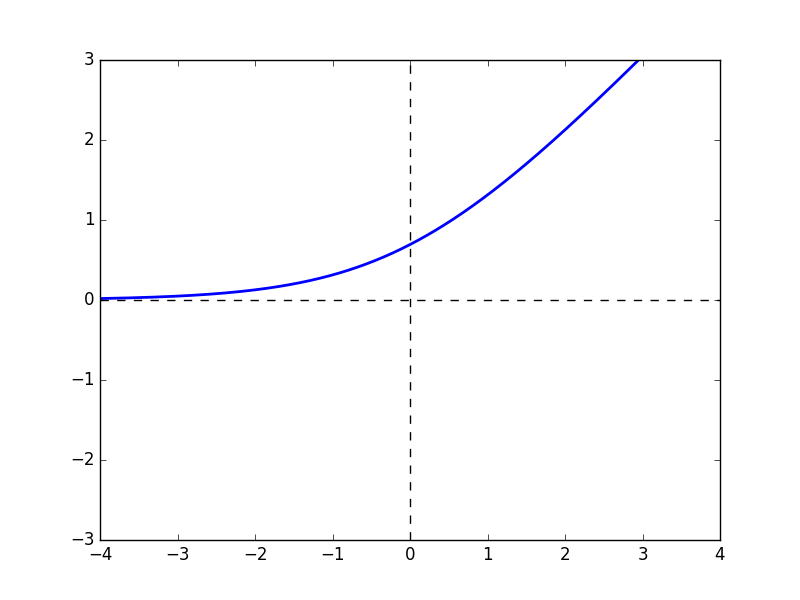
\includegraphics[width=\linewidth]{pics/act_soft_relu.png}
      \begin{center}
        {\bf Soft ReLU}
      \end{center}
      \[ \phi(z) = \log 1 + e^z \]
    \end{column}
  \end{columns}
\end{frame}

\begin{frame}{More Activation Functions}
  \begin{columns}
    \begin{column}{0.3 \linewidth}
      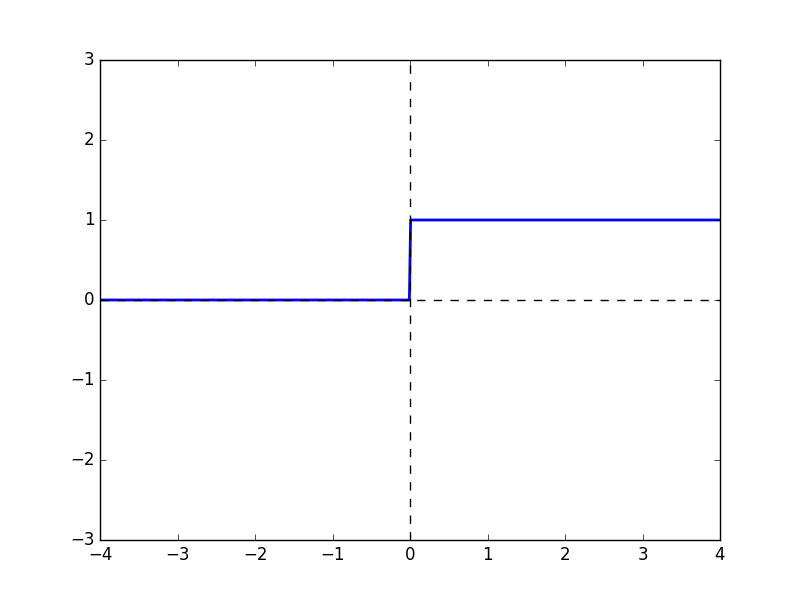
\includegraphics[width=\linewidth]{pics/act_threshold.png}
      \begin{center}
        {\bf Hard Threshold}
      \end{center}
      \[ \phi(z) = \left\{ \begin{array}{ll} 1 & \textrm{if } z > 0 \\ 0 & \textrm{if } z \leq 0 \end{array} \right. \]
    \end{column}

    \begin{column}{0.3 \linewidth}
      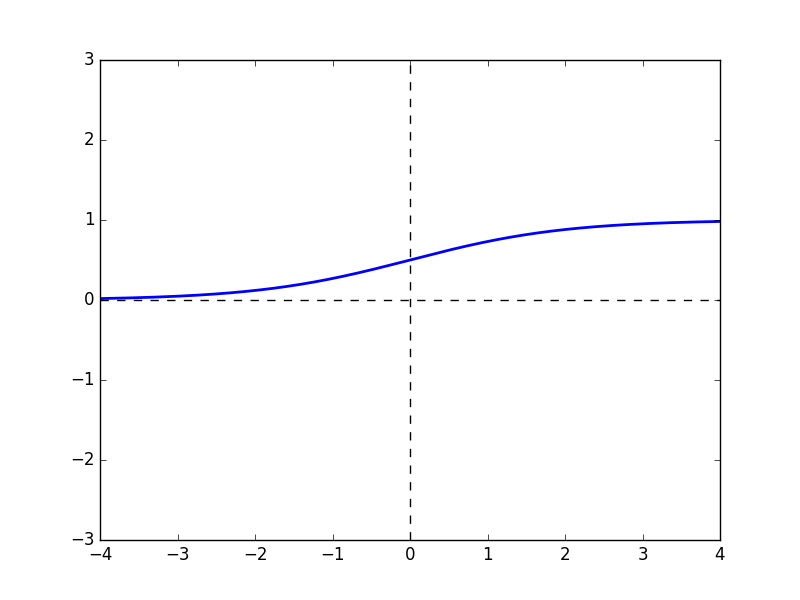
\includegraphics[width=\linewidth]{pics/act_logistic.png}
      \begin{center}
        {\bf Logistic}
      \end{center}
      \[ \phi(z) = \frac{1}{1+e^{-z}} \]
    \end{column}

    \begin{column}{0.3 \linewidth}
      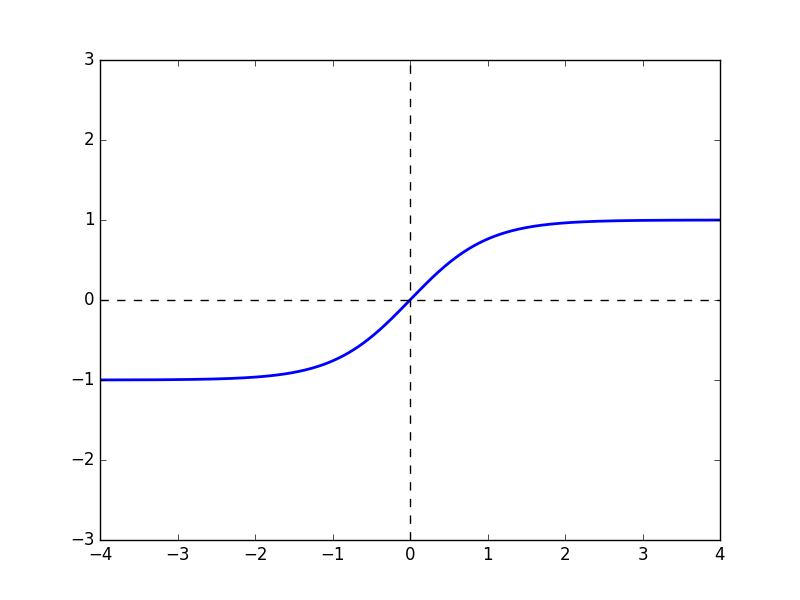
\includegraphics[width=\linewidth]{pics/act_tanh.png}
      \begin{center}
        {\bf Hyperbolic Tangent} \\
        {\bf (tanh)}
      \end{center}
      \[ \phi(z) = \frac{e^{z} - e^{-z}}{e^{z} + e^{-z}} \]
    \end{column}
  \end{columns}
\end{frame}


\begin{frame}{Computation in Each Layer}
\medskip 

\begin{columns}
\begin{column}{0.75\linewidth}
%\centering

Each layer computes a function.
\begin{align*}
          \mathbf{h}^{(1)} &= f^{(1)}(\x) = \phi(\mathbf{W}^{(1)} \x + \mathbf{b}^{(1)}) \\
          \mathbf{h}^{(2)} &= f^{(2)}(\mathbf{h}^{(1)}) = \phi(\mathbf{W}^{(2)} \mathbf{h}^{(1)} + \mathbf{b}^{(2)})\\
                       & \hspace{0.5em} \vdots \\
          \y &= f^{(L)}(\mathbf{h}^{(L-1)})
\end{align*}
\bigskip
\pause 
The network computes a composition of functions.\\[-7mm]
        \[ \y = f^{(L)} \circ \cdots \circ f^{(1)}(\x). \]

\pause{
The last layer depends on the task.
\begin{itemize}
\item Regression: \quad $\y = f^{(L)}(\mathbf{h}^{(L-1)}) = (\bs w^{(L)})^{\top} \mathbf{h}^{(L-1)} + b^{(L)}$
\item Classification:  $\y = f^{(L)}(\mathbf{h}^{(L-1)}) = \alert{\sigma\big(}(\bs w^{(L)})^{\top} \mathbf{h}^{(L-1)} + b^{(L)}\alert{\big)}$
\end{itemize}
}
\bigskip

\end{column}
\begin{column}{0.35\linewidth}
    \centering
      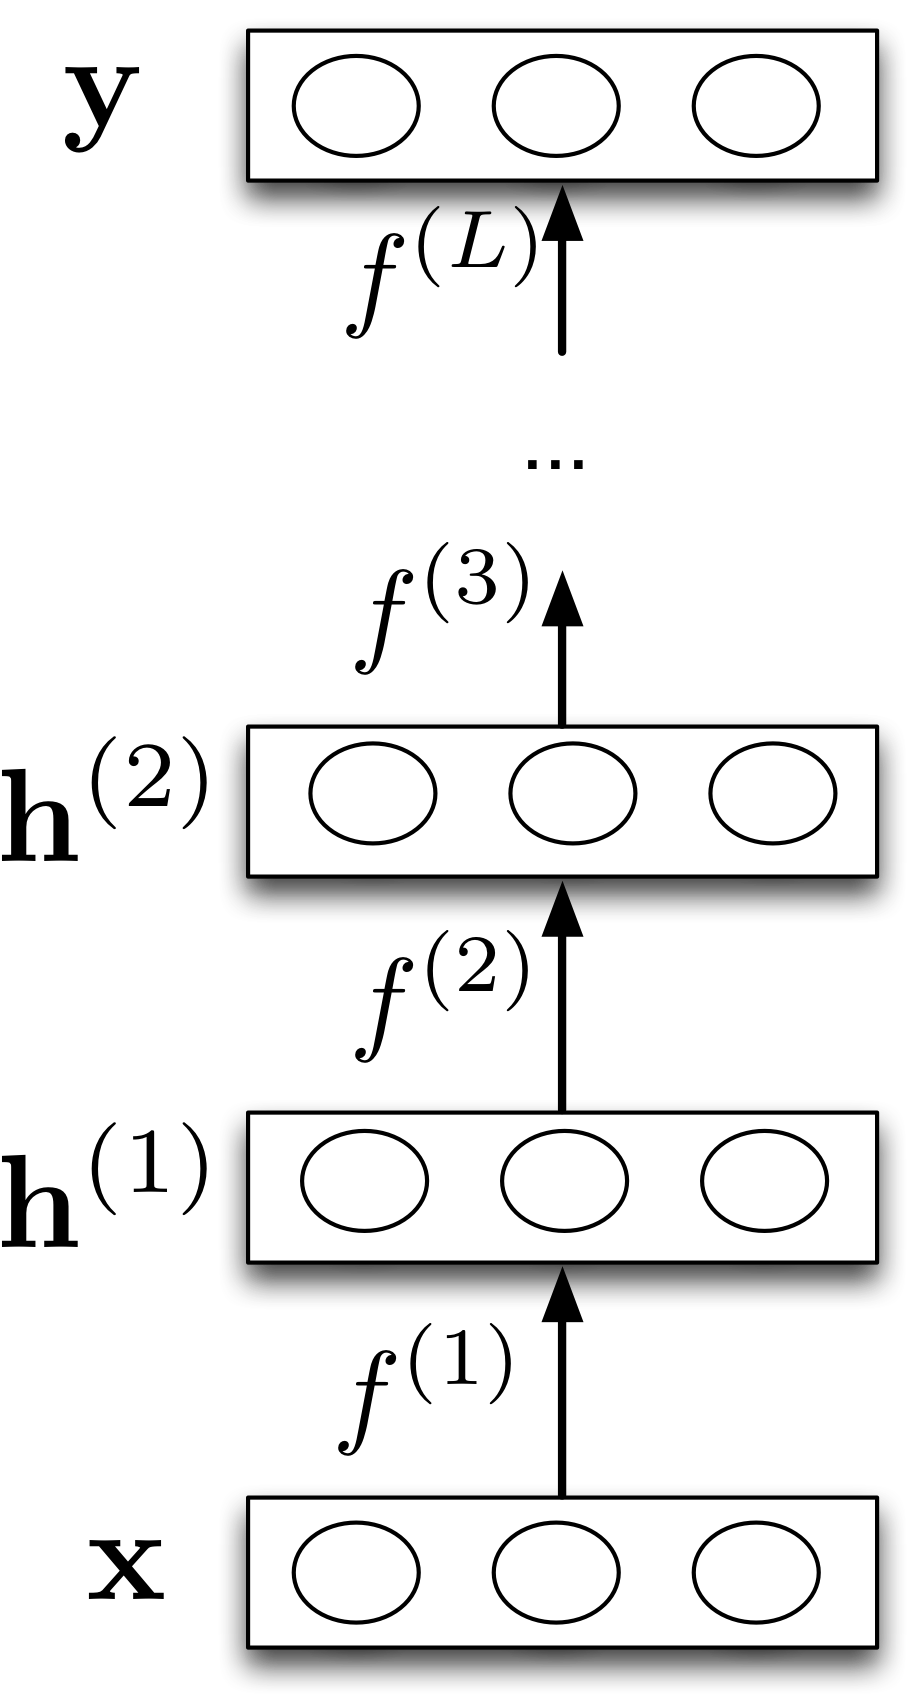
\includegraphics[width=.7\linewidth]{pics/layer_functions.png}
\end{column}
\end{columns}
\end{frame}


\begin{frame}{Expressive Power of Linear Networks}
  \begin{itemize}
  \setlength\itemsep{1em}
  \item Consider a linear layer: the activation function was the identity. The layer just computes an affine transformation of the input.
  \item Any sequence of linear layers is equivalent to a single linear layer.
    \[ \y = \underbrace{\bs W^{(3)} \bs W^{(2)} \bs W^{(1)}}_{\triangleq \mathbf{W}^\prime} \x \]
\item Deep linear networks can only represent linear functions 
--- no more expressive than linear regression.
  \end{itemize}
\end{frame}


\begin{frame}{Expressive Power of Non-linear Networks}
  \begin{itemize}
  \setlength\itemsep{1em}
    \item Multi-layer feed-forward neural networks  with non-linear activation functions
    \item \textbf{Universal Function Approximators}:  They can approximate any function arbitrarily well.
      %, \\
   % i.e., for any $f : \mathcal{X} \to \mathcal{T}$ there is a sequence $f_i \in \mathcal{H}$ with $f_i \to f$.
    \item True for various activation functions  (e.g. thresholds, logistic, ReLU, etc.)
  \end{itemize}
%      \begin{figure}
%      \centering
%      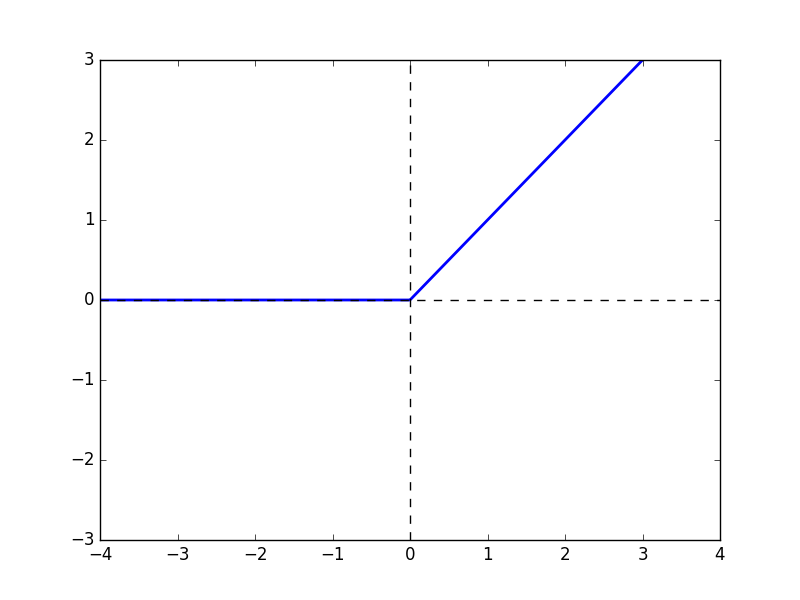
\includegraphics[width=0.4\linewidth]{pics/act_relu.png}
%      \end{figure}
\end{frame}


\begin{frame}{Learning Weights in a Neural Network}

\begin{itemize}
\item Goal is to learn weights in a multi-layer neural network 
using gradient descent.
\medskip

\item Weight space for a multi-layer neural net: one set of weights for each unit in every layer of the network
\medskip

\item Define a loss $\mathcal L(\bs t,\y)=\mathcal L(\bs t,\y(\x,\bs w))$ and compute the gradient of the cost $$E(\bs w)\;=\;\tfrac1N\sum_{n=1}^N \mathcal L(\bs t_n,\y(\x_n,\bs w)),$$
which is the average loss over all the training examples.
\medskip
\item To calculate $\nabla E ( \bs w)$ efficiently we use backpropagation. (we omit details here)
\end{itemize}
\end{frame}


\section{Autoencoders}

\begin{frame}{}
	\begin{center}
		\alert{{\Huge Autoencoders}}
	\end{center}
\end{frame}

\begin{frame}{Non-linear Dimension Reduction}
  \begin{tabular}{ll}  
    \begin{tabular}{l}
      \!\!\!\!\!\!  \!\!\!\!\!\!       \!\!\!\!\!\!       \!\!\!\!\!\!       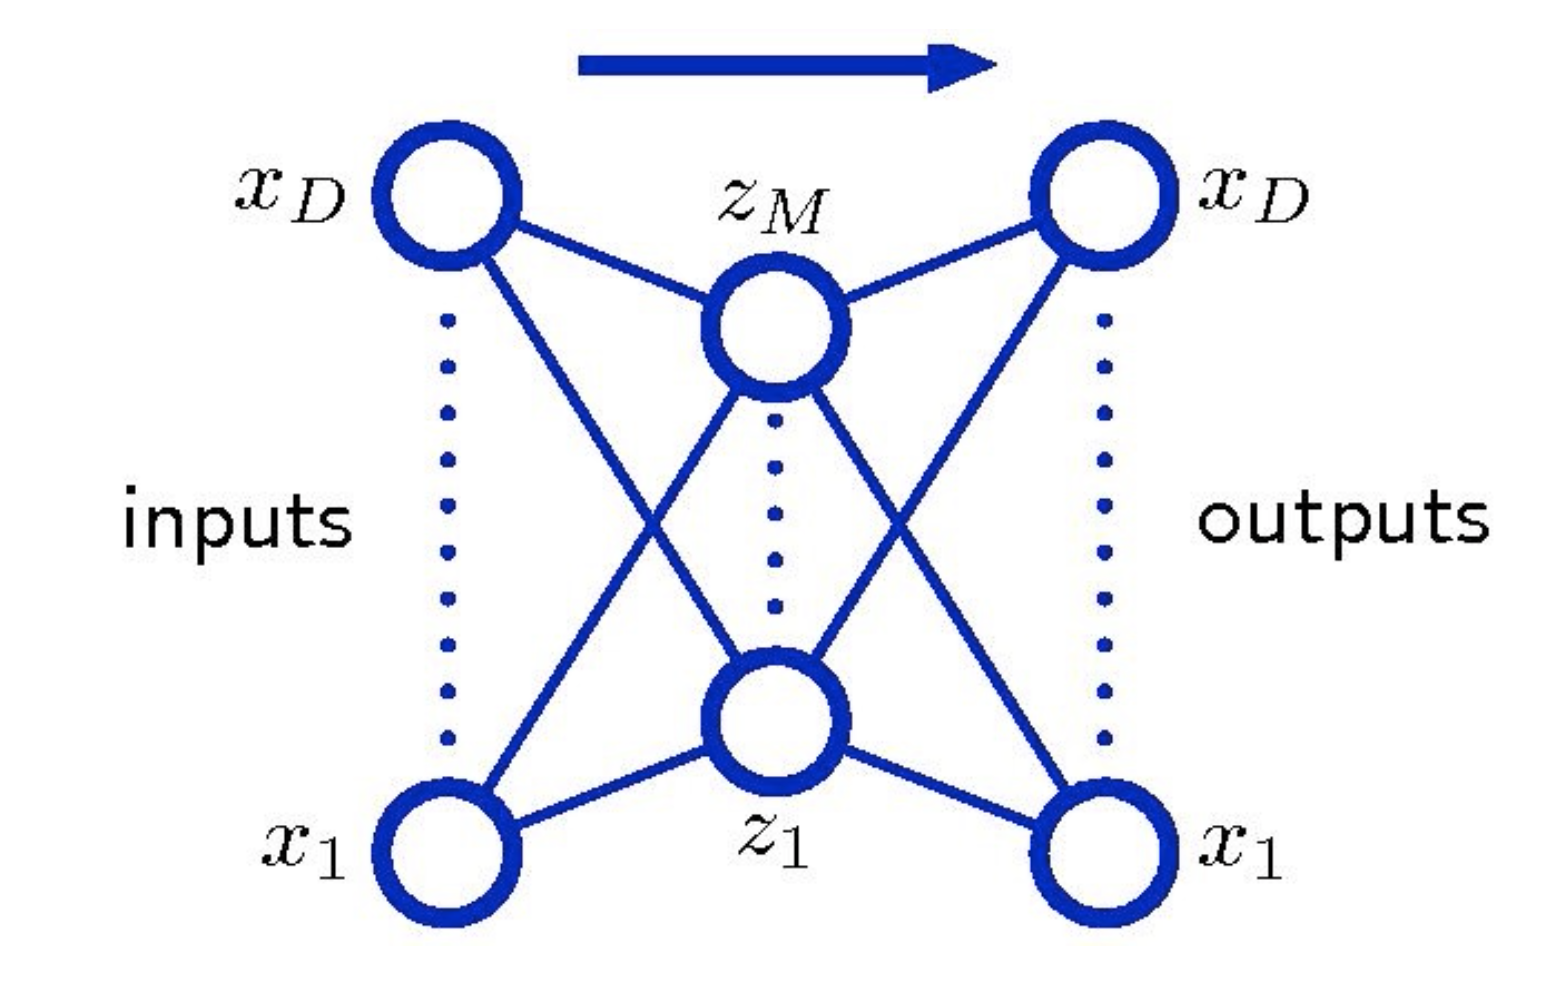
\includegraphics[width=1.9in]{pics/2-layer-auto-enc.png}
    \end{tabular}
    & \begin{tabular}{l}
        \hspace{-.4in} \parbox{.75\linewidth}{
        \begin{itemize}
        \item Neural networks can be used for \alert{nonlinear dimensionality reduction}.\\[3mm]
        \item This is achieved by having the same number of outputs as inputs. These models are called autoencoders.\\[3mm]
        \pause
        \item Consider a feed-forward neural network that has $D$ inputs, $D$ outputs, and $M$ hidden units, with $M<D$.\\[3mm]
        \item We can squeeze the information through a bottleneck.\\[3mm]
        \pause
        \item If we use a linear network (linear activation) this is very similar to Principal Components Analysis.
        \end{itemize}
        }
      \end{tabular}  
  \end{tabular}
\end{frame}


\begin{frame}
  \frametitle{Autoencoders and PCA}
  \begin{itemize}
  \item Given an input $\boldsymbol x$, its corresponding reconstruction is given by:
    $$
    y_k(\boldsymbol x, \boldsymbol w) = \sum_{j=1}^M w_{kj}^{(2)} \sigma\Big(\sum_{i=1}^D w_{ji}^{(1)}x_i \Big), \ \ \ k=1,...,D.
    $$
  \item We learn the parameters $\boldsymbol w$ by minimizing the reconstruction error:\\[-2mm]
    $$
    E(\boldsymbol w) = \frac{1}{2N} \sum_{n=1}^{N} \| y(\boldsymbol x_n, \boldsymbol w) - \boldsymbol x_n \|^2
    $$
  \end{itemize}
\pause
\vspace{-2mm}
  \begin{tabular}{ll}  
    \begin{tabular}{l}
      \!\!\!\!\!\! \!\!\!\!\!\! \!\!\!\!\!\! \!\!\!\!\!\!      \!\!\!\!\!\!       \!\!\!\!\!\!       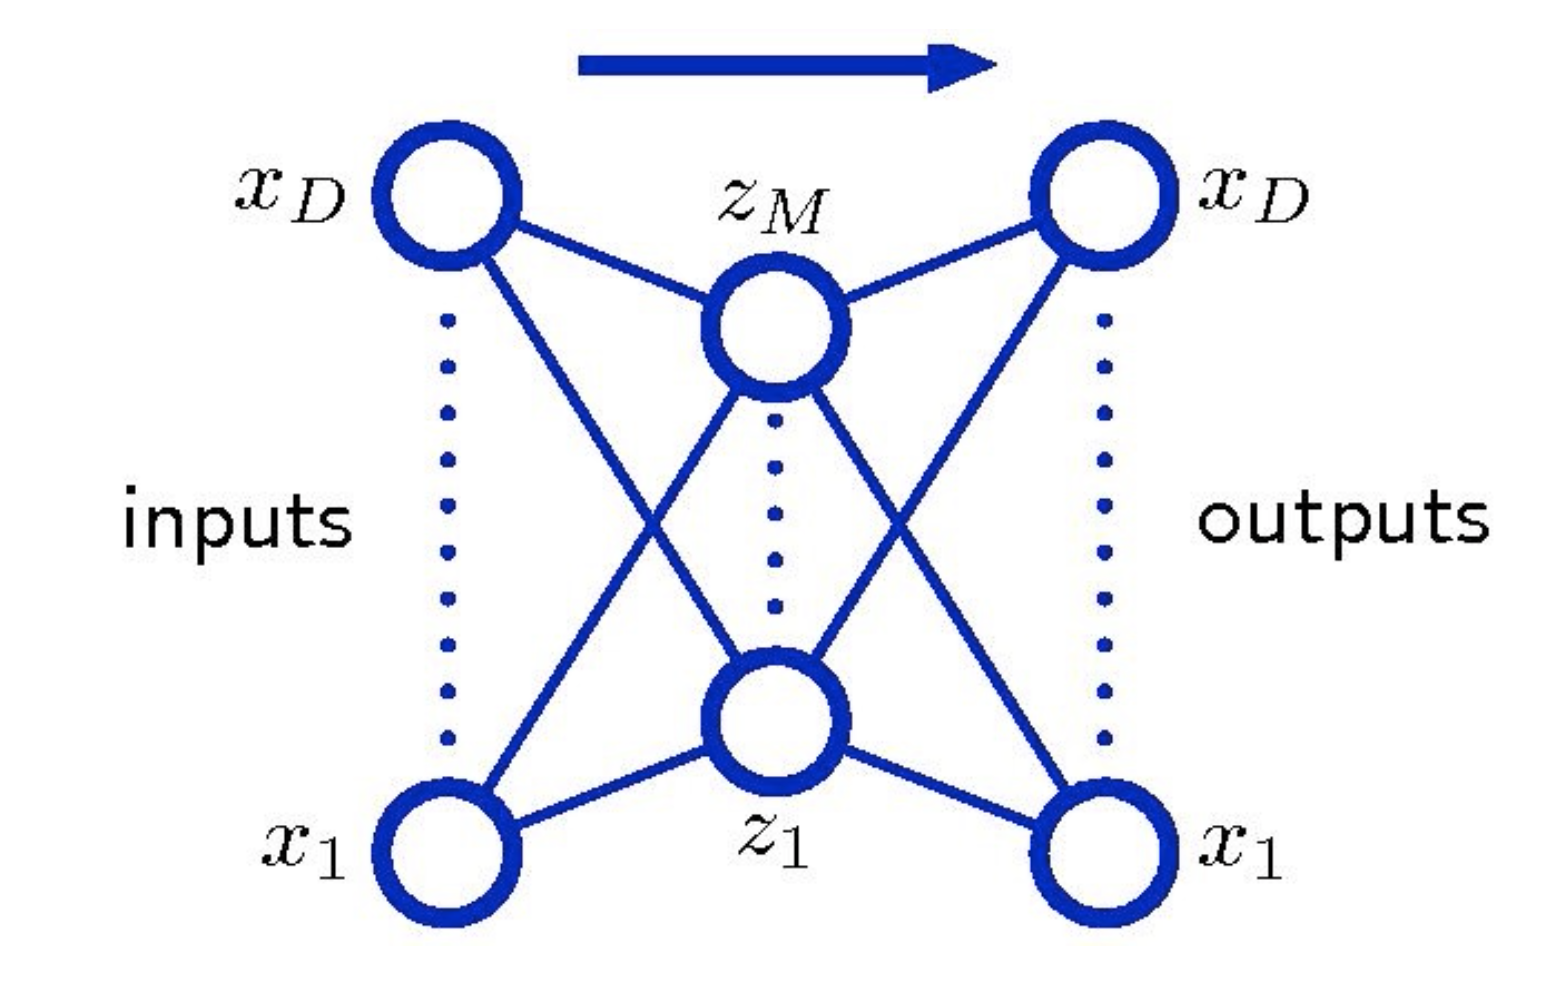
\includegraphics[width=1.99in]{pics/2-layer-auto-enc.png}
    \end{tabular}
    & \begin{tabular}{l}
        \hspace{-.4in} \parbox{.75\linewidth}{
        \begin{itemize}
        \item In the case when layers are \alert{linear}:
        \begin{itemize}
        \item it will learn hidden units that are linear functions of the data and minimize squared error.
        \item $M$ hidden units will span the same space as the first $M$ principal components (PCA). 
        \end{itemize}      
        \end{itemize}
        }
      \end{tabular}  
  \end{tabular}
\end{frame}

\begin{frame}
  \frametitle{Deep Autoencoders }
  \begin{tabular}{ll}  
    \begin{tabular}{l}
      \!\!\!\!\!\!      \!\!\!\!\!\!       \!\!\!\!\!\!       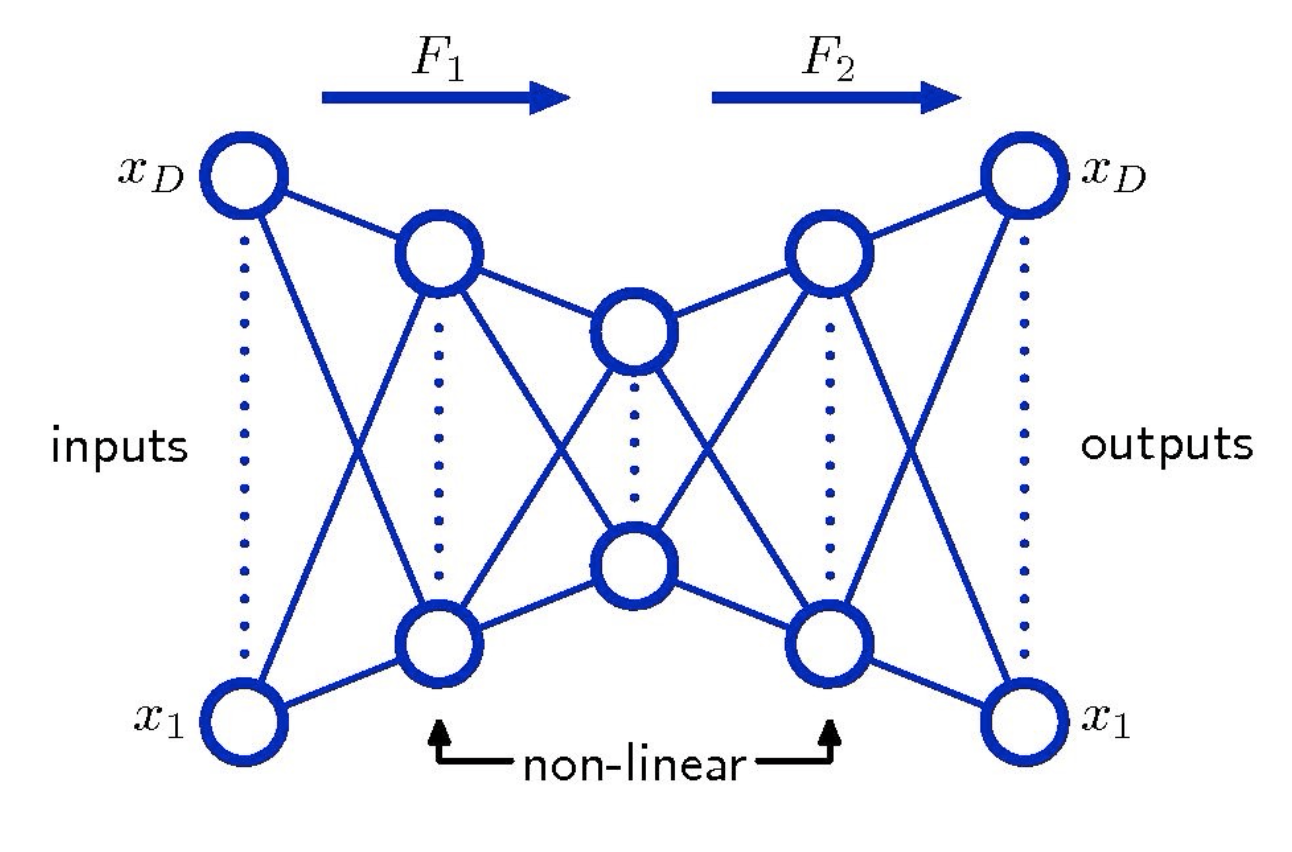
\includegraphics[width=1.99in]{pics/deep-auto-enc.png}
    \end{tabular}
    & \begin{tabular}{l}
        \hspace{-.4in} \parbox{.7\linewidth}{
        
        \begin{itemize}
        \item We can put extra nonlinear hidden layers between the input and the bottleneck and between the bottleneck and the output.\\[3mm]
        \item This gives nonlinear generalization of PCA, providing non-linear dimensionality reduction.\\[3mm]
\pause
        \item The network can be trained by the minimization of the reconstruction error function.\\[3mm]
        \item Much harder to train.
          
        \end{itemize}

        }
      \end{tabular}  \\
  \end{tabular}
\end{frame}


\begin{frame}
  \frametitle{Geometrical Interpretation}

  \begin{itemize}
  \item Geometrical interpretation of the mappings performed by the network with 2 hidden layers for the case of $D=3$ and $M=2$ units in the middle layer.
    \begin{figure}
      \centering
      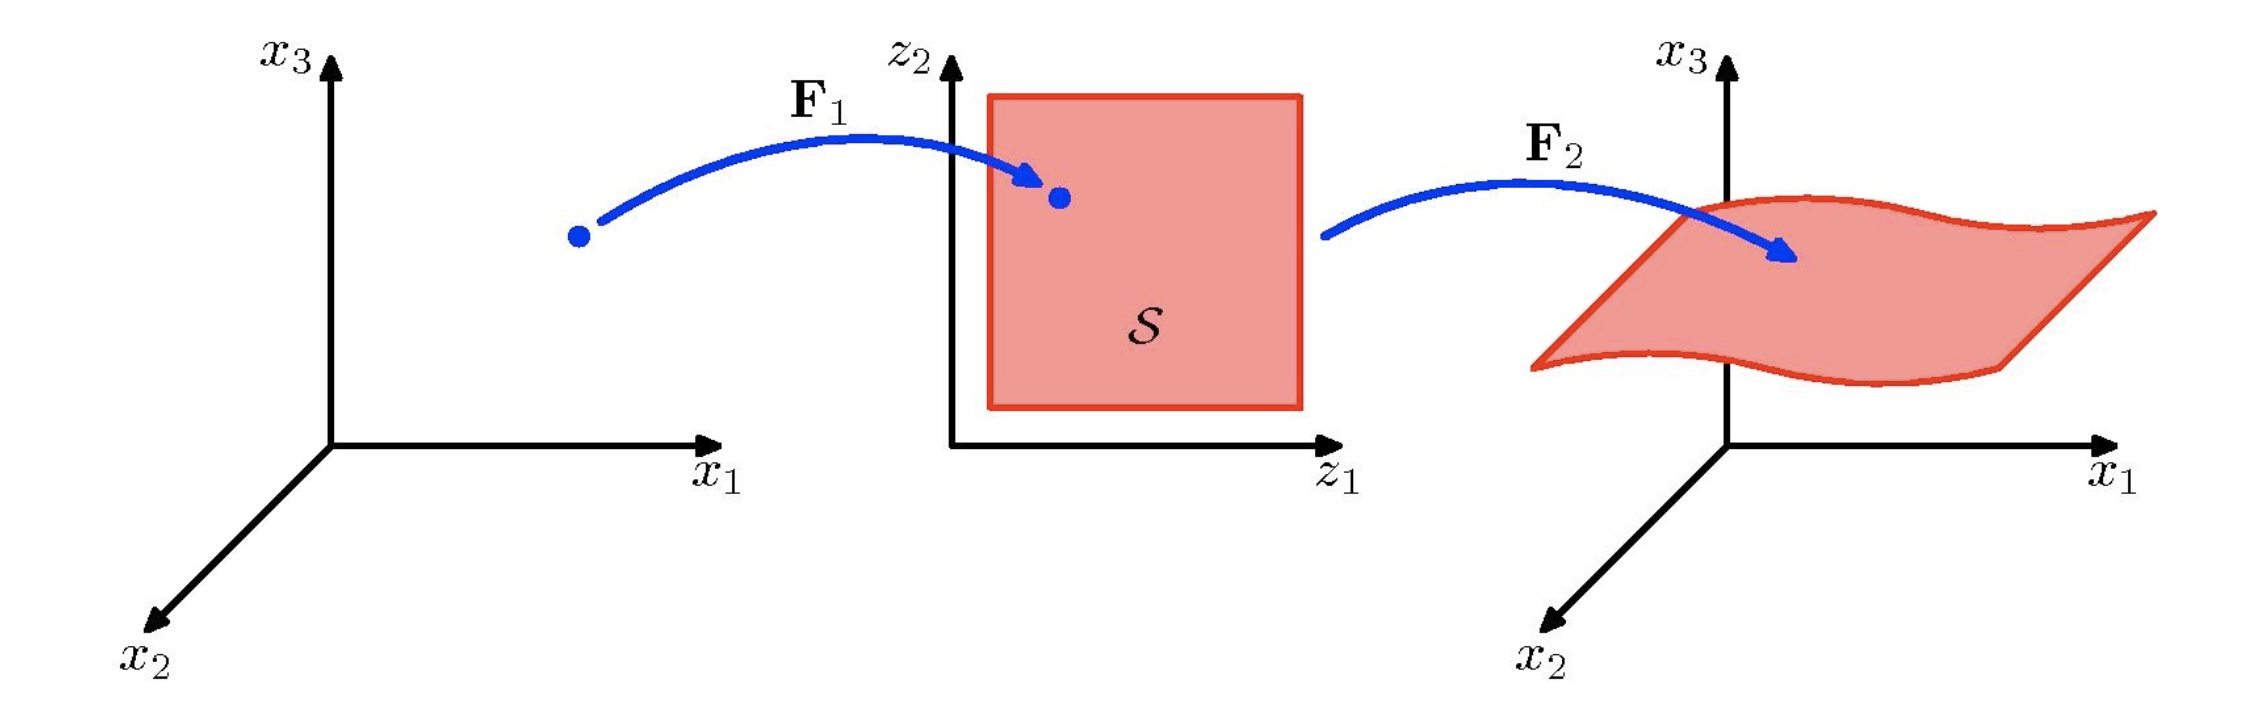
\includegraphics[width=3.99in]{pics/geo-inter.png}
    \end{figure}
  \item The mapping $F_1$ defines a nonlinear projection of points in the original $D$-space into the $M$-dimensional subspace.
  \item The mapping $F_2$ maps from an $M$-dimensional space into $D$-dimensional space.
  \end{itemize}
\end{frame}

\begin{frame}{Deep Autoencoders}
  \begin{tabular}{ll}  
    \begin{tabular}{l}
      \!\!\!\!\!\!      \!\!\!\!\!\!       \!\!\!\!\!\!       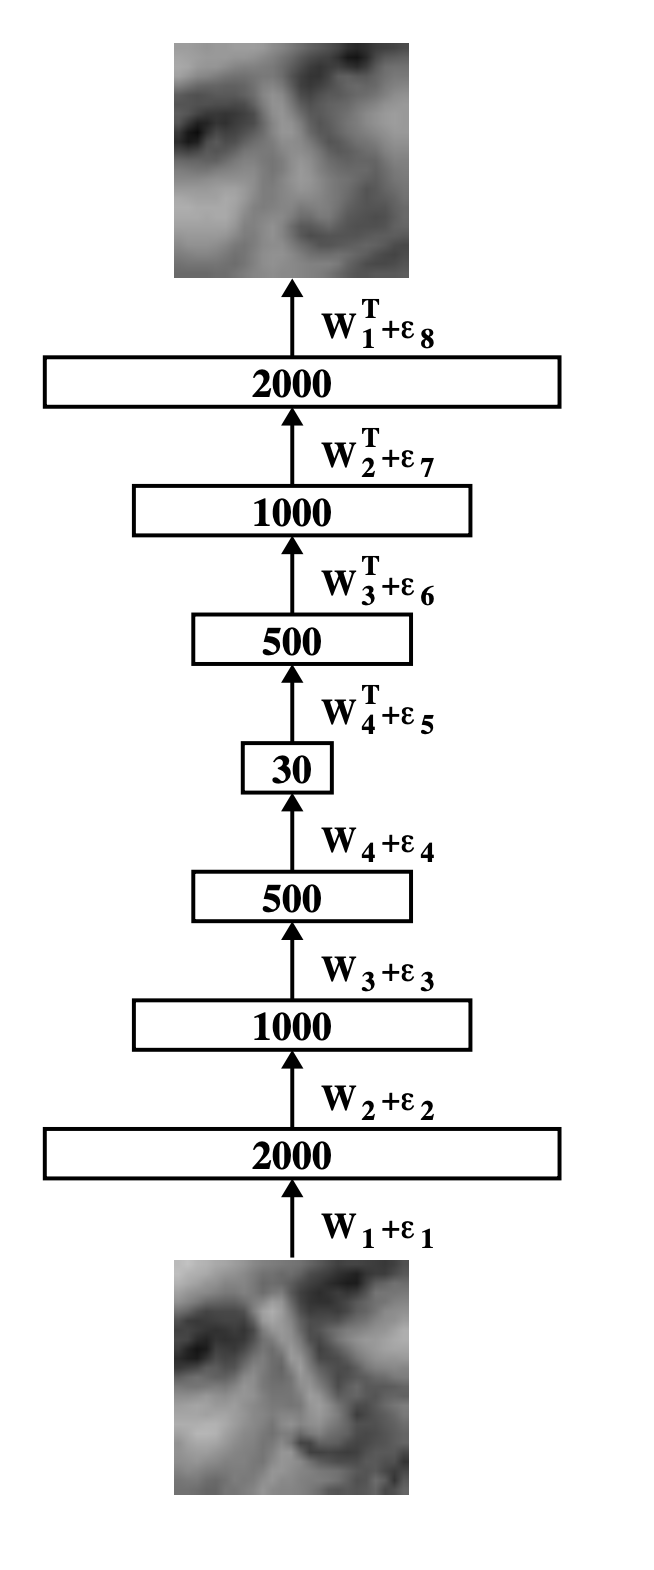
\includegraphics[width=0.99in]{pics/auto-enc-face.png}
    \end{tabular}
    & \begin{tabular}{l}
        \hspace{-.4in} \parbox{.7\linewidth}{
        
        \begin{itemize}
        \item[] \begin{figure}
            \centering
            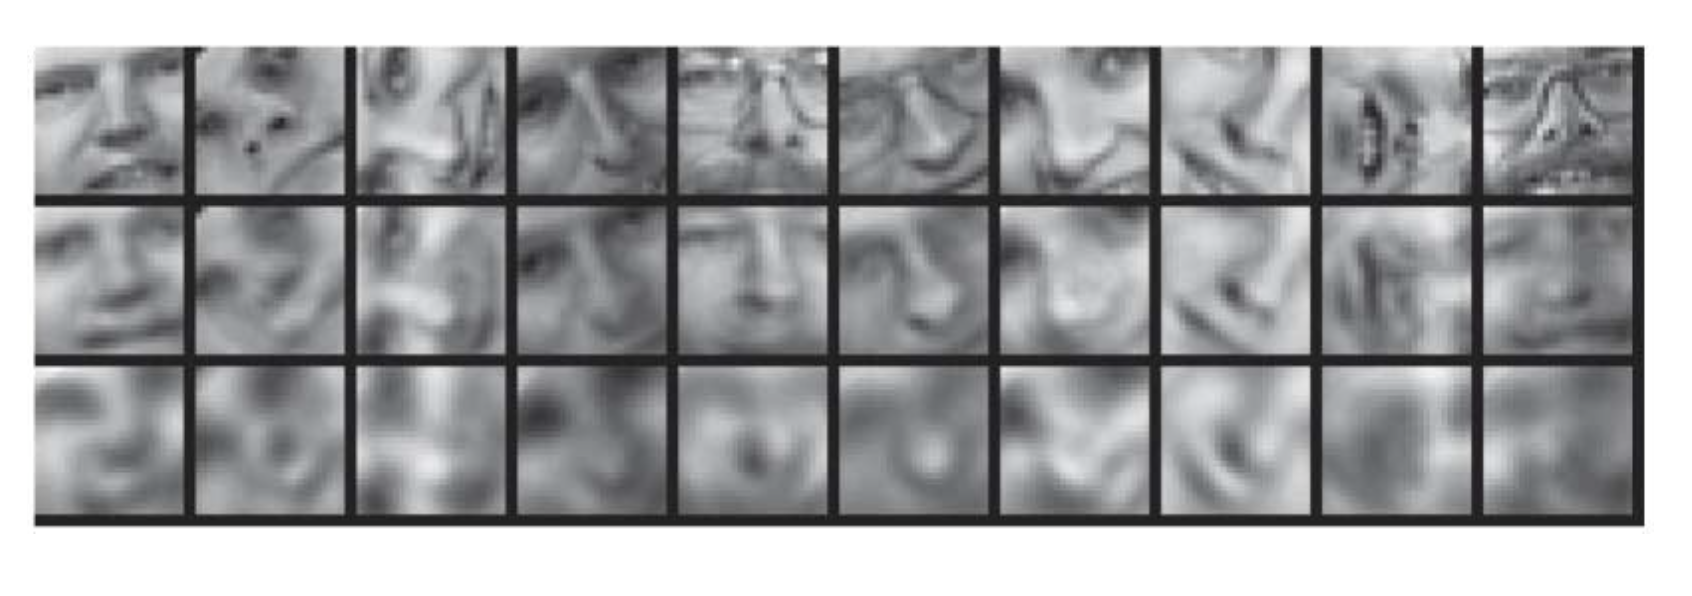
\includegraphics[width=2.99in]{pics/auto-enc-faces.png}
          \end{figure}
        \item We can consider very deep autoencoders.
%        \item There is an efficient way to learn these deep autoencoders.
        \item By row: Real data, Deep autoencoder with a bottleneck of 30 units, and 30-d PCA.      
        \end{itemize}
        }
      \end{tabular}  \\
  \end{tabular}
\end{frame}

\begin{frame}{Deep Autoencoders}
  \begin{itemize}
  \item Similar model for MNIST handwritten digits:
    \begin{figure}
      \centering
      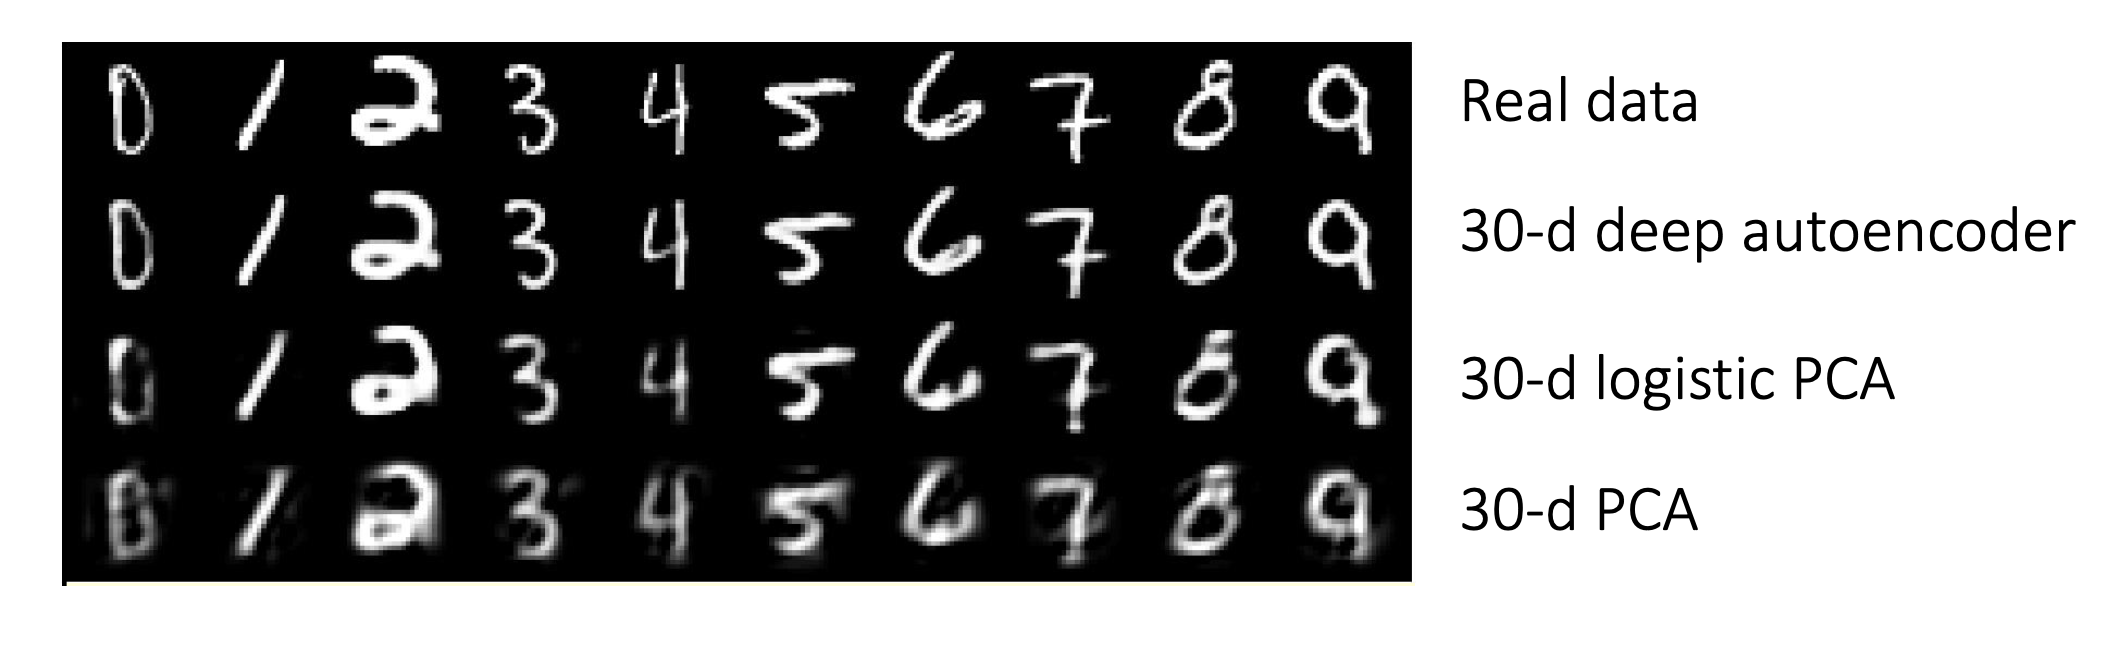
\includegraphics[width=3.99in]{pics/auto-enc-mnist.png}
    \end{figure}
  \item Deep autoencoders tend to produce better reconstructions.
  \item Of course, they are much more involved computationally.
  \end{itemize}
\end{frame}


\begin{frame}{Autoencoders: Summary}
  Autoencoders reconstruct their input via an encoder and a decoder.


  \begin{itemize}
  \item \textbf{Encoder}:  $e(x) = z \in F, \quad x \in X$

  \item \textbf{Decoder}:  $d(z) = \tilde x \in X$
  \item where  $X$ is the data space, and  $F$ is the feature (latent) space.
  

\item  $z$ is the code, 
\pause
 compressed representation of the input,  $x$. It is important that this code is a bottleneck, i.e. that
  $$
  \text{dim} \ F \ll \text{dim} \ X
  $$
\item Goal:
  $  \tilde x \;=\; d(e(x)) \;\approx\; x$.
\end{itemize}
\vspace{-9mm}\hspace{8mm}\qquad\qquad\qquad\qquad\qquad\qquad\qquad    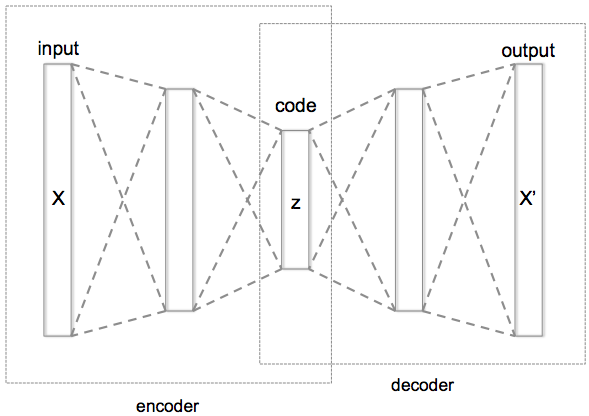
\includegraphics[width=1.8in]{pics/lecture_10_1.png}
\end{frame}


\begin{frame}
  \frametitle{Issues with (deterministic) Autoencoders}

  \begin{itemize}
  \item \textbf{Issue 1}: Proximity in data space does not mean proximity in feature space
    \begin{itemize}
    \item The codes learned by the model are deterministic, i.e.
      $$
      \begin{aligned}
        g(x_1) = z_1 \quad\Longrightarrow\quad f(z_1) = \tilde x_1 \\
        g(x_2) = z_2 \quad\Longrightarrow\quad f(z_2) = \tilde x_2 
      \end{aligned}
      $$

   \item but proximity in feature space is not ``directly'' enforced for inputs in close proximity in data space, i.e.
      $$
x_1 \approx x_2\quad\not\!\Longrightarrow  \quad     z_1 \approx z_2 
      $$

    \item The latent space may not be continuous, or allow easy interpolation.


    \end{itemize}
  \end{itemize}
\end{frame}


\begin{frame}{One issue}
Proximity in data space does not mean proximity in feature space.
    \begin{itemize}
    \item If the space has discontinuities (eg. gaps between clusters), the decoder may generate unrealistic outputs.

      \begin{figure}
      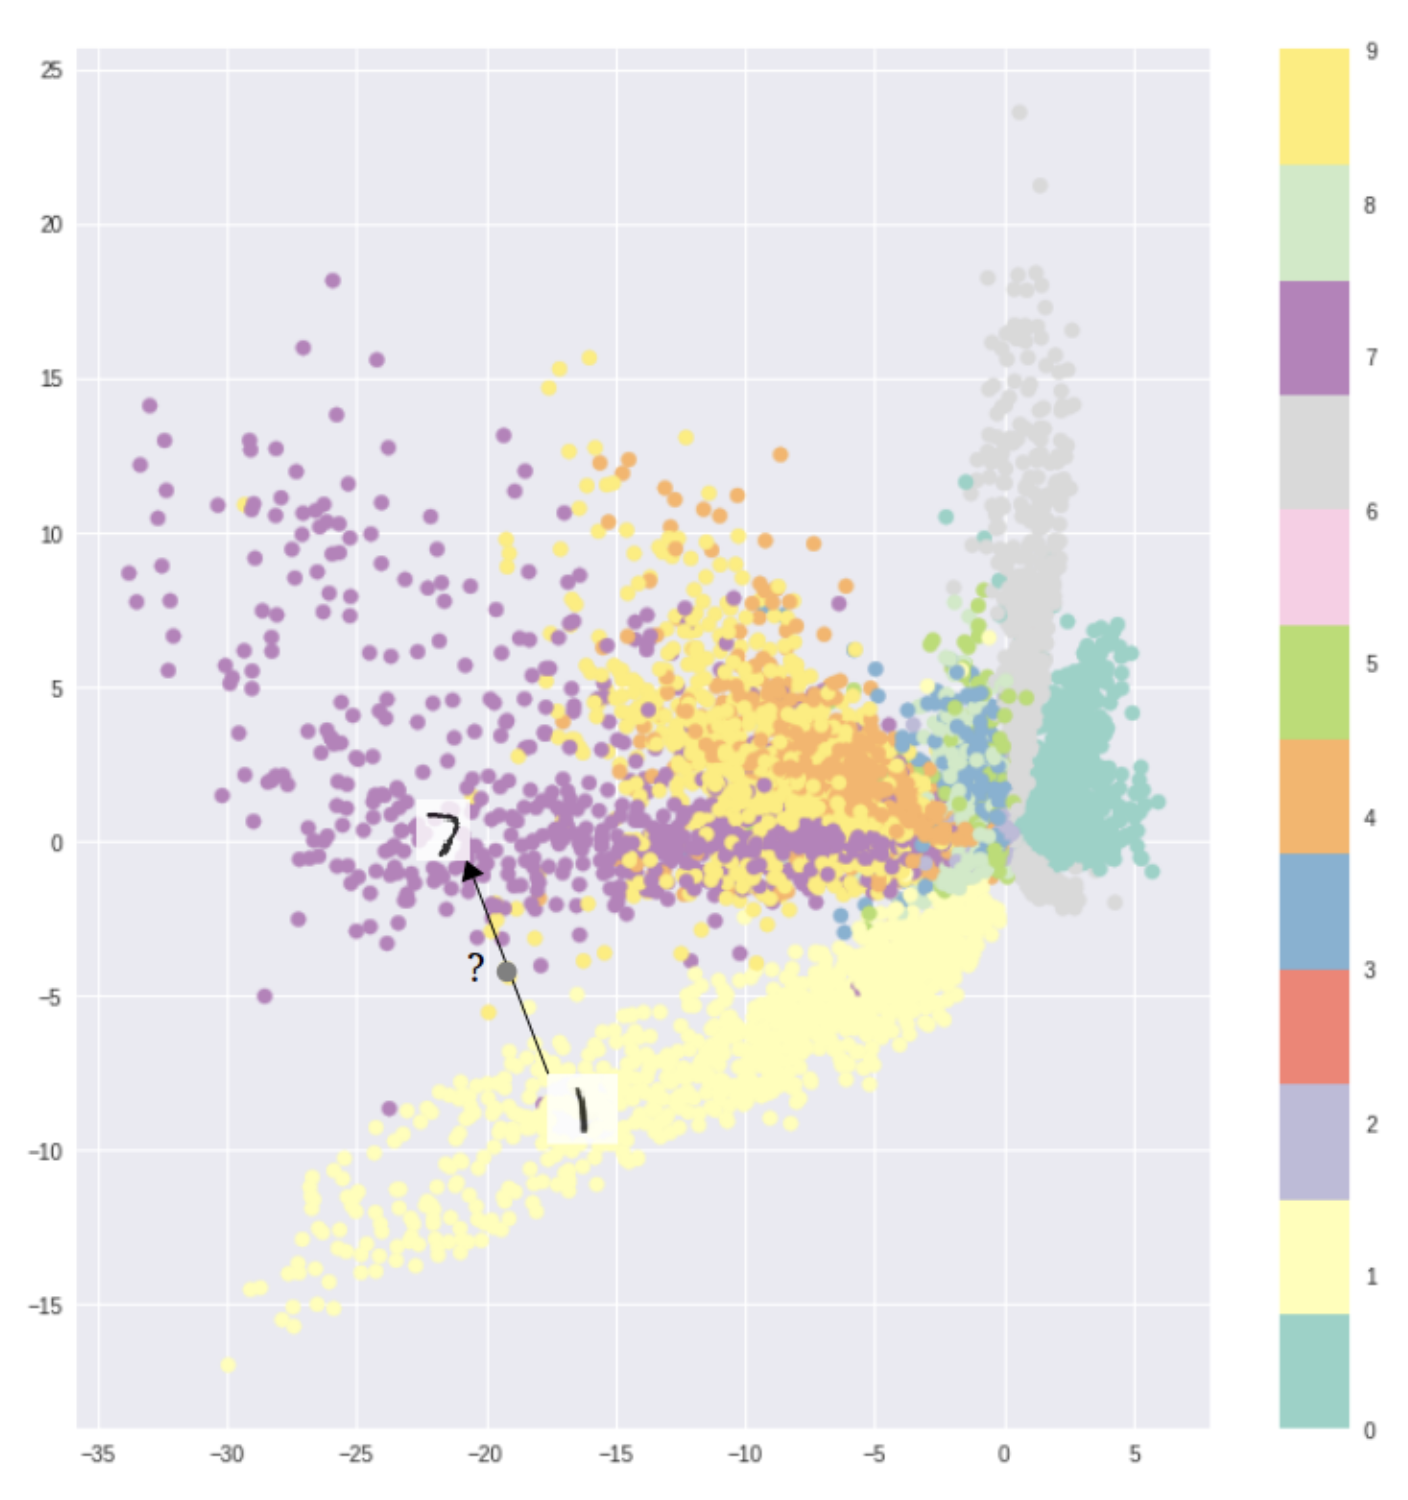
\includegraphics[width=1.9in]{pics/mnist-ae}
%        \includegraphics[width=4in]{pics/cluster-vae.png}  
      \end{figure}
    \end{itemize}

  {\tiny Two dimensional latent space for the MNIST digit data.(Image credit: I.~Shafkat)}
\end{frame}





\end{document}

